% !TEX root = perelman-geometry.tex
%!TEX TS-program = pdflatex
%!TEX encoding = UTF-8 Unicode

\setchapterpreamble[o]{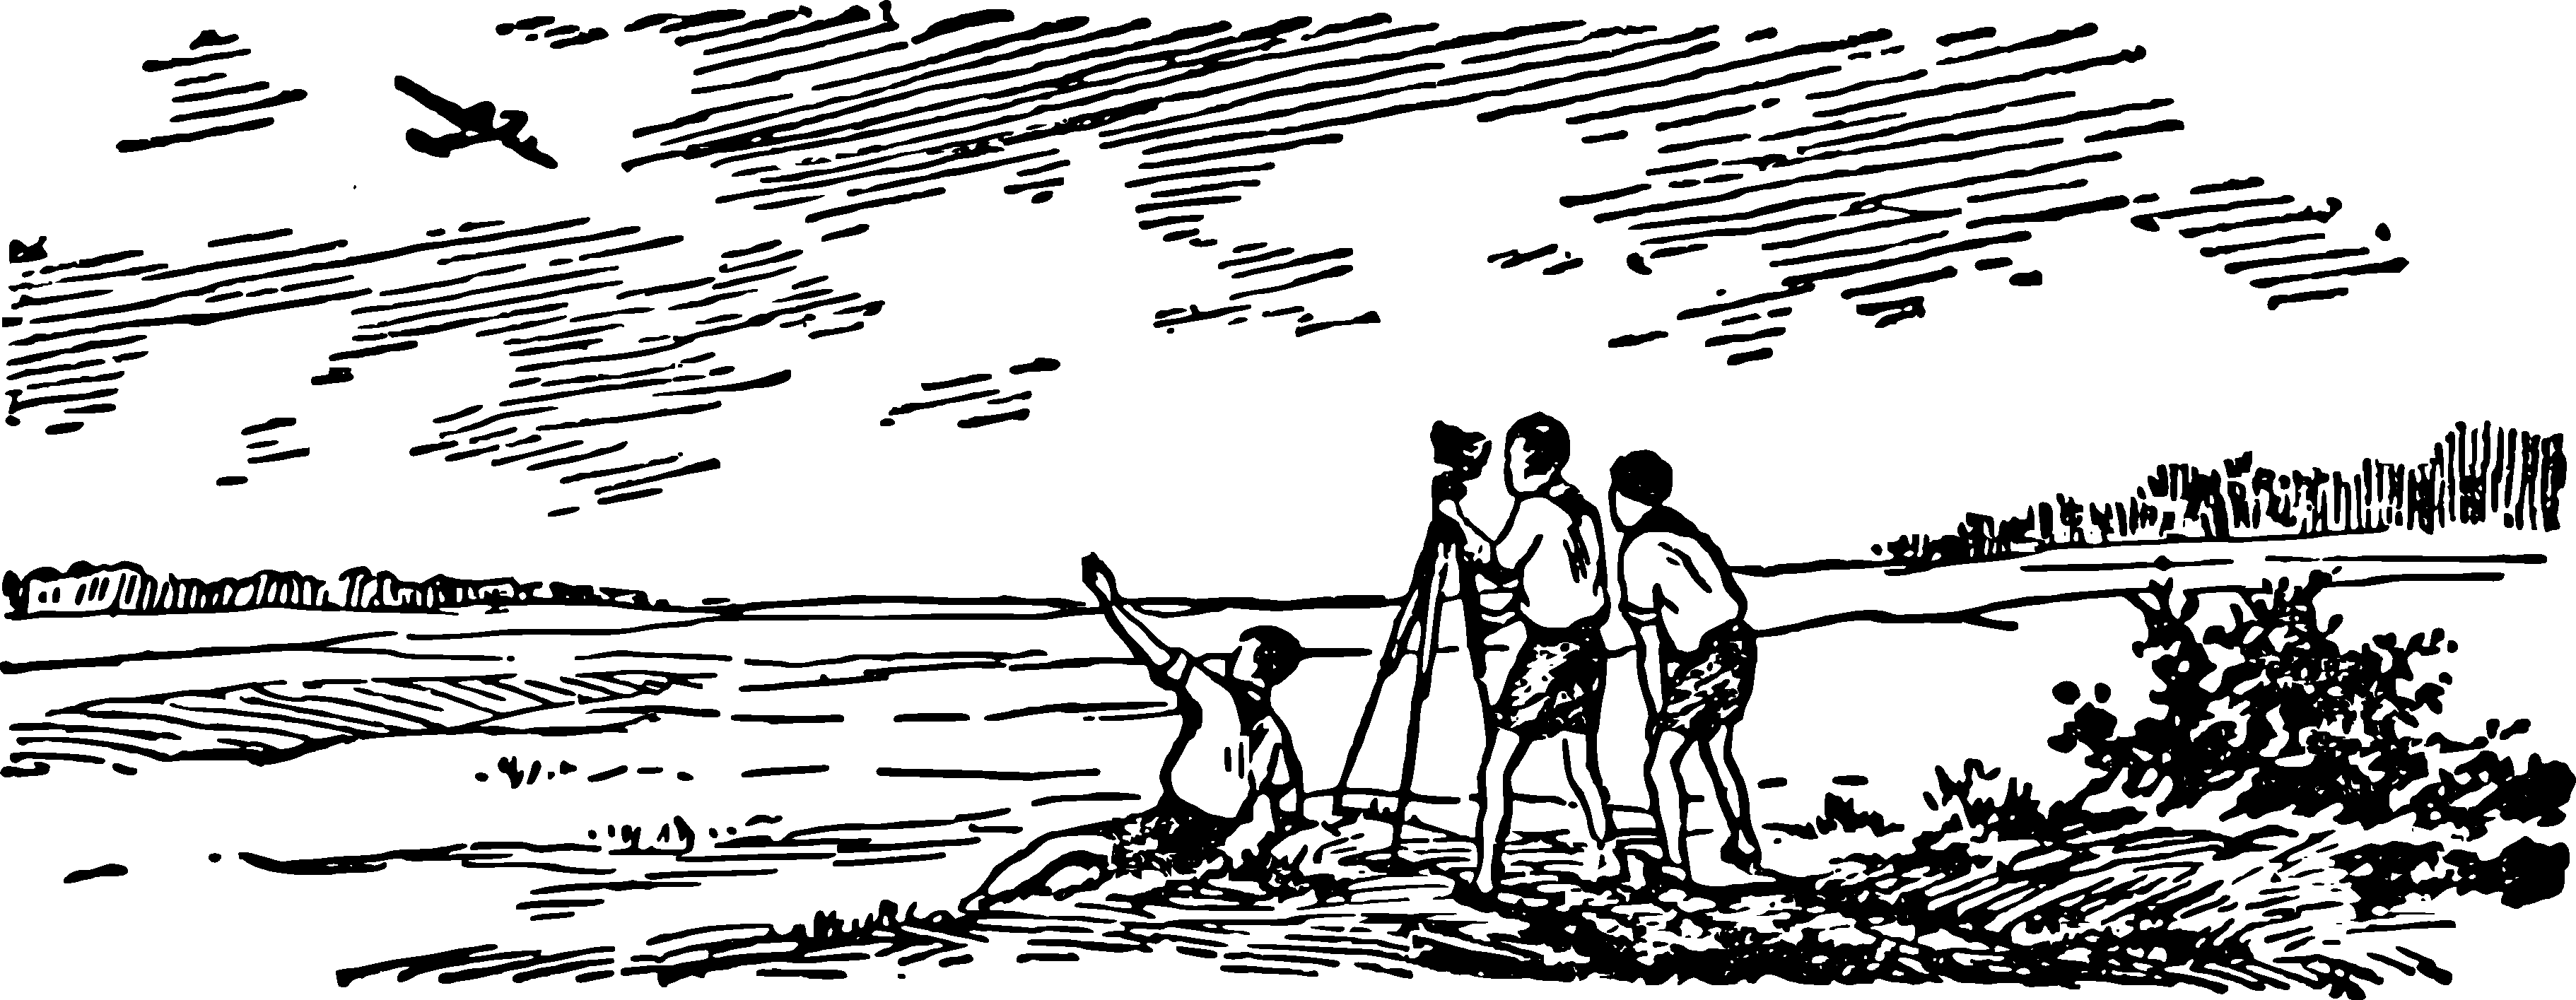
\includegraphics[width=1.2\textwidth]{figures/ch-03/fig-ch-03-head.pdf}\bigskip}

\chapter{Geometry In The Open Field}
\label{ch-03}

\section{Visible sizes of the Moon}
\label{sec-3.1}


What size does the full moon in the sky seem to you? Different people give quite different answers to this question.

Estimates like ``the size of a plate,'' ``the size of an apple,'' ``the size of a human face,'' and so on, are extremely vague, indefinite, indicating only that those answering do not understand the essence of the question.

The correct answer to such an apparently ordinary question can only be given by someone who clearly understands what exactly needs to be understood by the ``apparent'' or ``visible'' size of an object. Few suspect that here we are referring to the magnitude of a certain angle -- precisely the angle formed by two straight lines drawn to our eye from the extreme points of the object under consideration; this angle is called the ``angle of view'' or ``angular size of the object'' (\figr{fig-061}). 

\begin{figure}[h!]
\centering
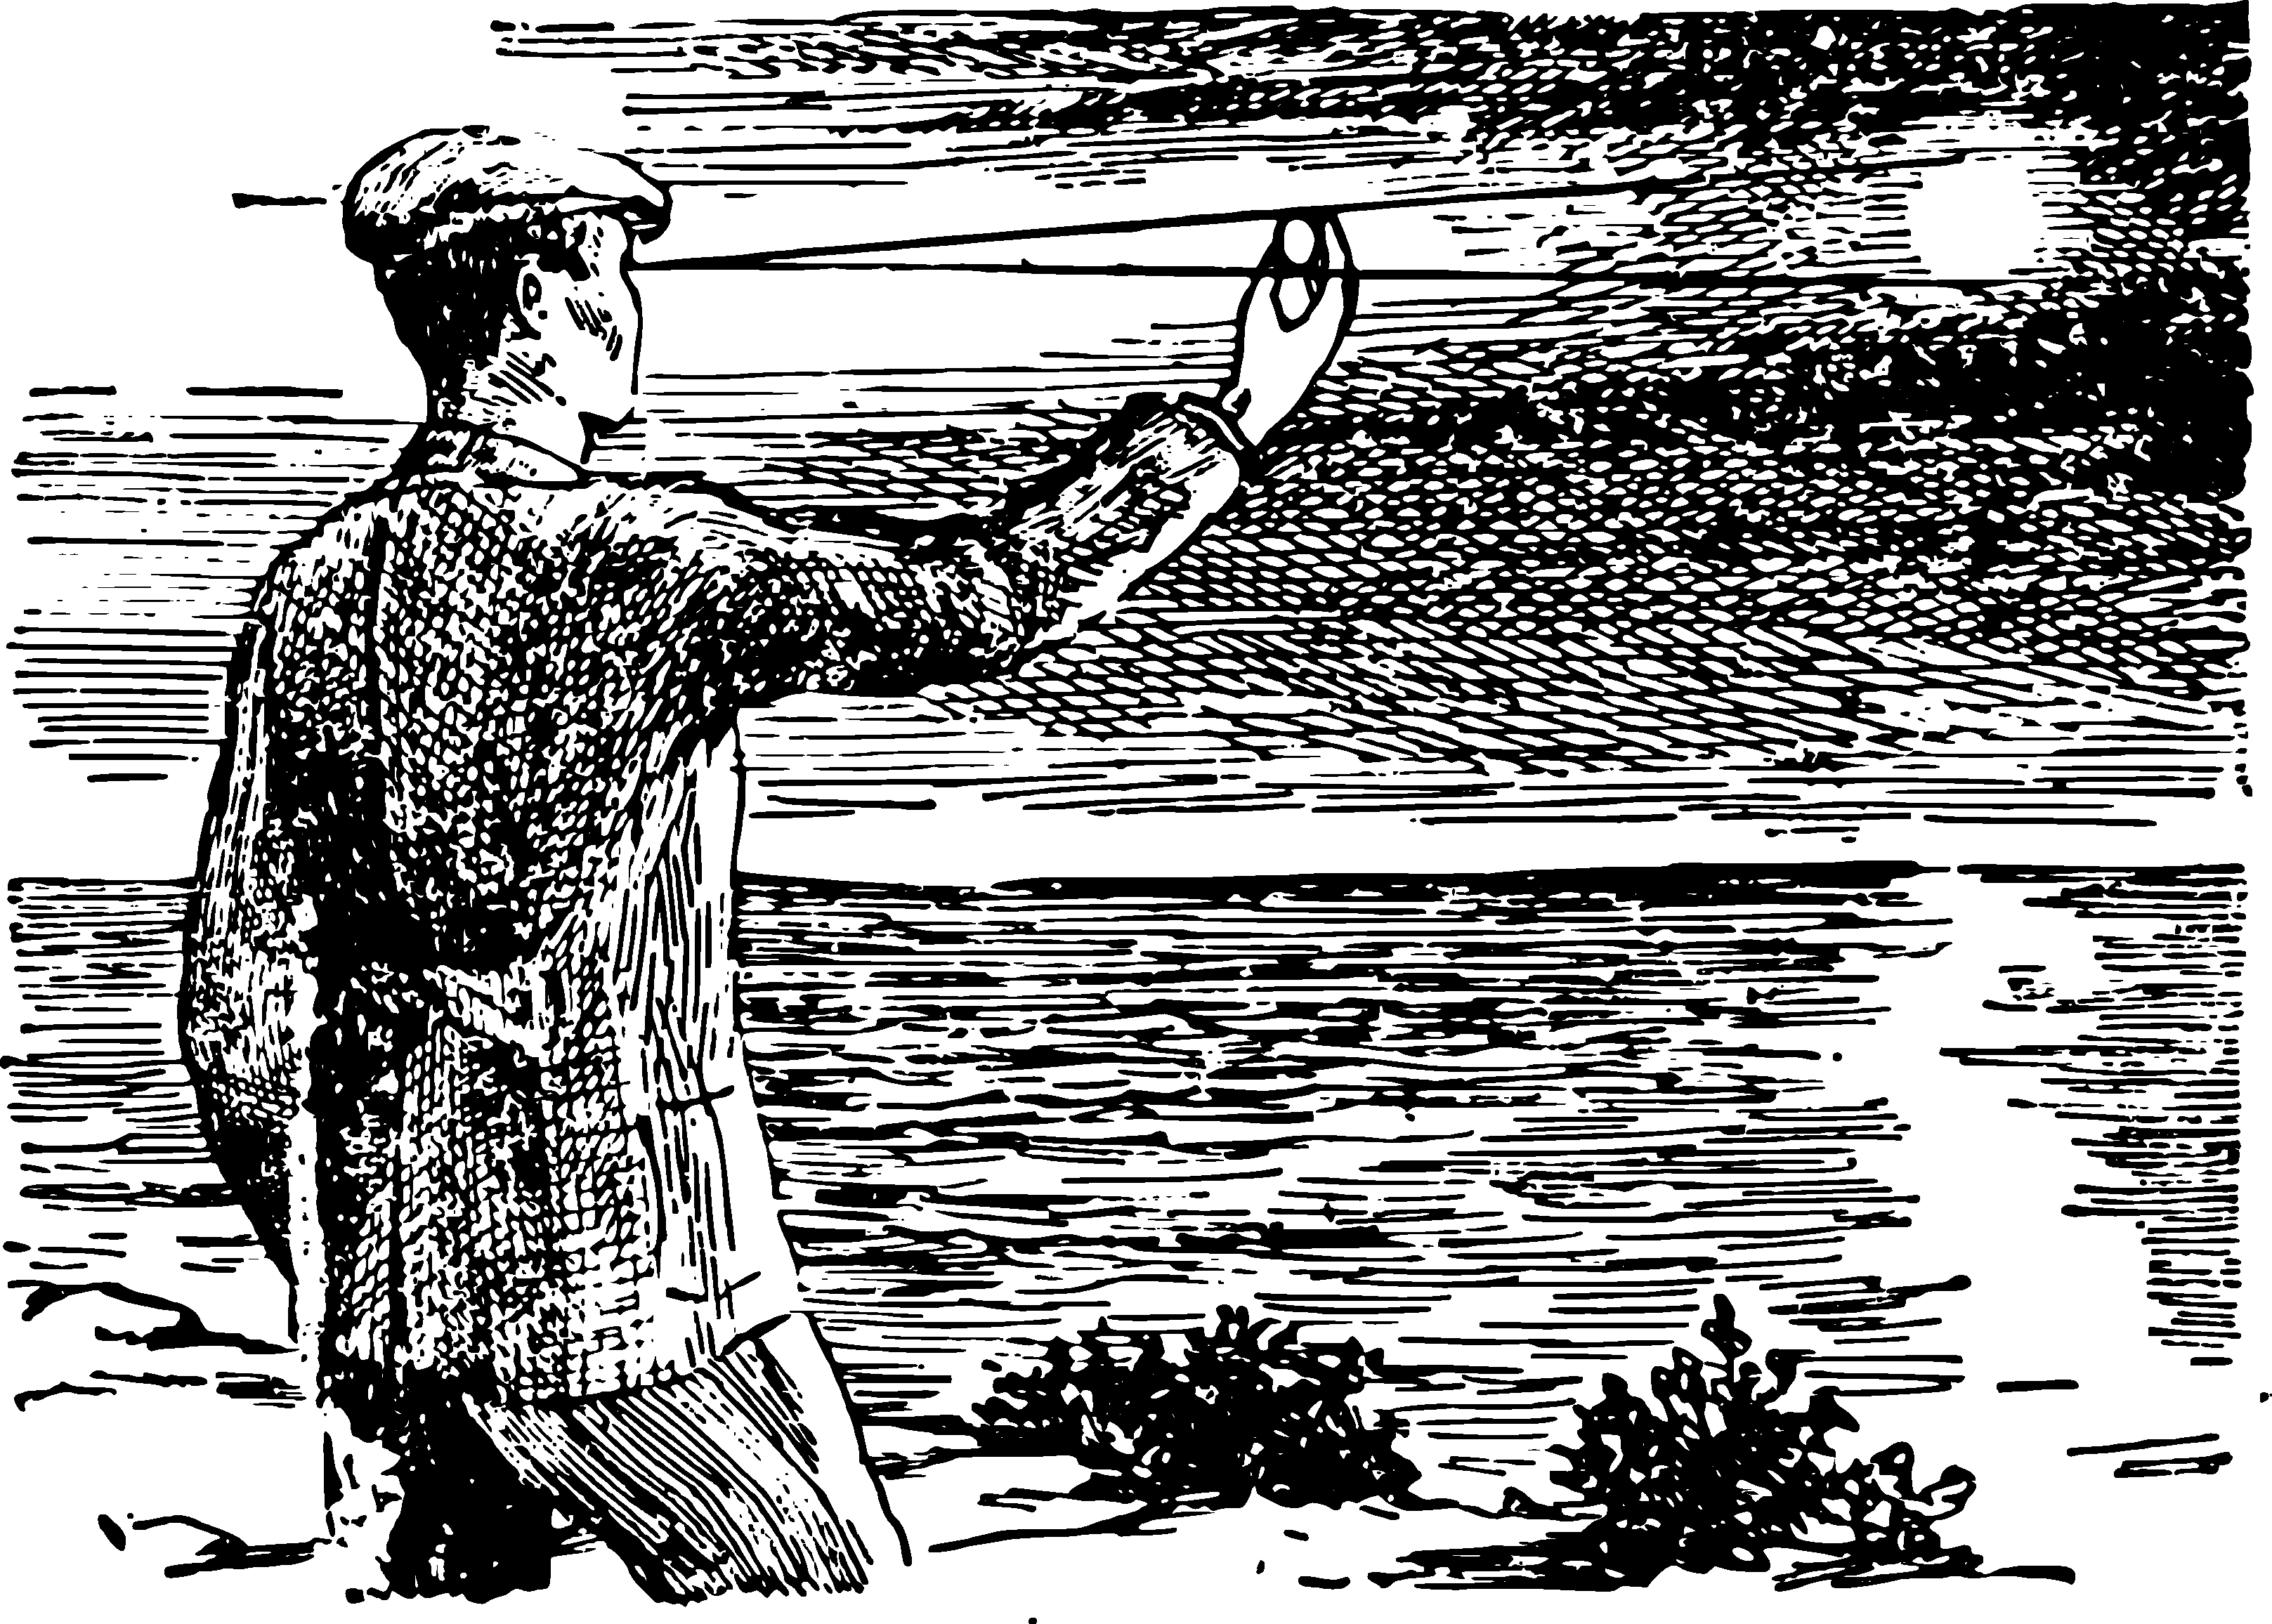
\includegraphics[width=0.9\textwidth]{figures/ch-03/fig-061.pdf}
\sidecaption{What is the angle of view or angular size of the object.\label{fig-061}}
\end{figure}

And when the apparent size of the Moon in the sky is assessed by comparing it with the sizes of a plate, an apple, and so forth, such answers are either completely meaningless or should imply that the Moon is visible in the sky at the same angle as the plate or apple. But such an indication alone is still insufficient: after all, we see a plate or an apple under different angles depending on their distance: up close -- under larger angles, far away -- under smaller ones. To introduce clarity, it is necessary to specify from what distance the plate or apple is being observed. Comparing the sizes of distant objects with the sizes of others, the distance of which is not indicated, is a very common literary technique employed by even first-rate writers. It creates a certain impression due to its closeness to the familiar psychology of most people, but it does not produce a clear image\ldots{} Here's an example from Shakespeare's \emph{King Lear}; it describes (by Edgar) the view from a high cliff by the sea:
\begin{quote}
\emph{How terrifying! How my head spins!\\
How low to cast my gaze\ldots{}\\
The rooks and crows that flutter there in the air at mid-distance,\\ Seem barely as large as flies. Halfway down Hangs a man gathering seaweed\dots{} \\
What a dreadful trade! He seems to me no bigger than his head.\\
The fishermen walking along the shore -- like mice;\\
and that tall ship at anchor has shrunk to the size of its boat;\\ its boat -- a floating dot, As if too small for sight\dots{}}
\end{quote}
These comparisons would provide a clear idea of distance if accompanied by indications of the degree of remoteness of the objects being compared (mice, the human head, crows, boat \dots{}). Similarly, when comparing the size of the moon with that of a plate or apples, indications of how far these everyday objects should be from the eye are necessary.

This distance turns out to be much greater than commonly thought. Holding an apple at arm's length, you not only obscure the Moon but also a significant portion of the sky. Suspend the apple on a string and gradually move away from it until it just covers the full lunar disk: in this position, the apple and the Moon will have the same apparent size for you. By measuring the distance from your eye to the apple, you will find that it is approximately 10 meters. This is how far you would need to move the apple away from you for it to truly seem to be the same size as the Moon in the sky! A plate, on the other hand, would need to be moved about 80 meters away from you, or about fifty steps.

What is said may seem unbelievable to anyone hearing it for the first time; however, it is indisputable and follows from the fact that we perceive the Moon at an angle of only \emph{half a degree}. We rarely have to estimate angles in our everyday lives, and therefore most people have a very vague idea of the magnitude of an angle with a small number of degrees, such as an angle of \ang{1}, \ang{29}, or \ang{59} (not to mention surveyors, draftsmen, and other specialists accustomed to practically measuring angles). We only estimate large angles more or less reasonably, especially if we manage to compare them with angles familiar to us between the hands of a clock; everyone, of course, is familiar with angles of \ang{90}, \ang{60}, \ang{30}, \ang{120}, \ang{150}, which we are so accustomed to seeing on a dial (at 8 o'clock, 2 o'clock, 1 o'clock, 4 o'clock, 5 o'clock) that even without distinguishing the numbers, we guess the time based on the size of the angle between the hands. But we usually see small and individual objects at much smaller angles and therefore completely lack the ability to even approximately estimate angles of view.


\section{Angle of View}
\label{sec-3.2}

To provide a concrete example of a one-degree angle, let's calculate how far an average-height person (1.7 meters) should move away from us to appear at such an angle. Translating the problem into the language of geometry, let's say we need to calculate the radius of a circle, the arc of which at \ang{1} has a length of 1.7 meters (strictly speaking, not an arc, but a chord, but for small angles, the difference between the lengths of the arc and the chord is negligible). We reason as follows: if the arc at \ang{1} equals 1.7 meters, then the full circumference containing \ang{360} will have a length of $1.7 \times 360 = \SI{610}{\meter}$, and the radius will be $1/2\pi$ the length of the circumference; if we take the value of $\pi$ as approximately 22/7, then the radius will be equal to
\begin{equation*}%
 \frac{610}{44/7} \approx \SI{98}{\meter}.
\end{equation*}
\begin{figure}[h!]
\centering
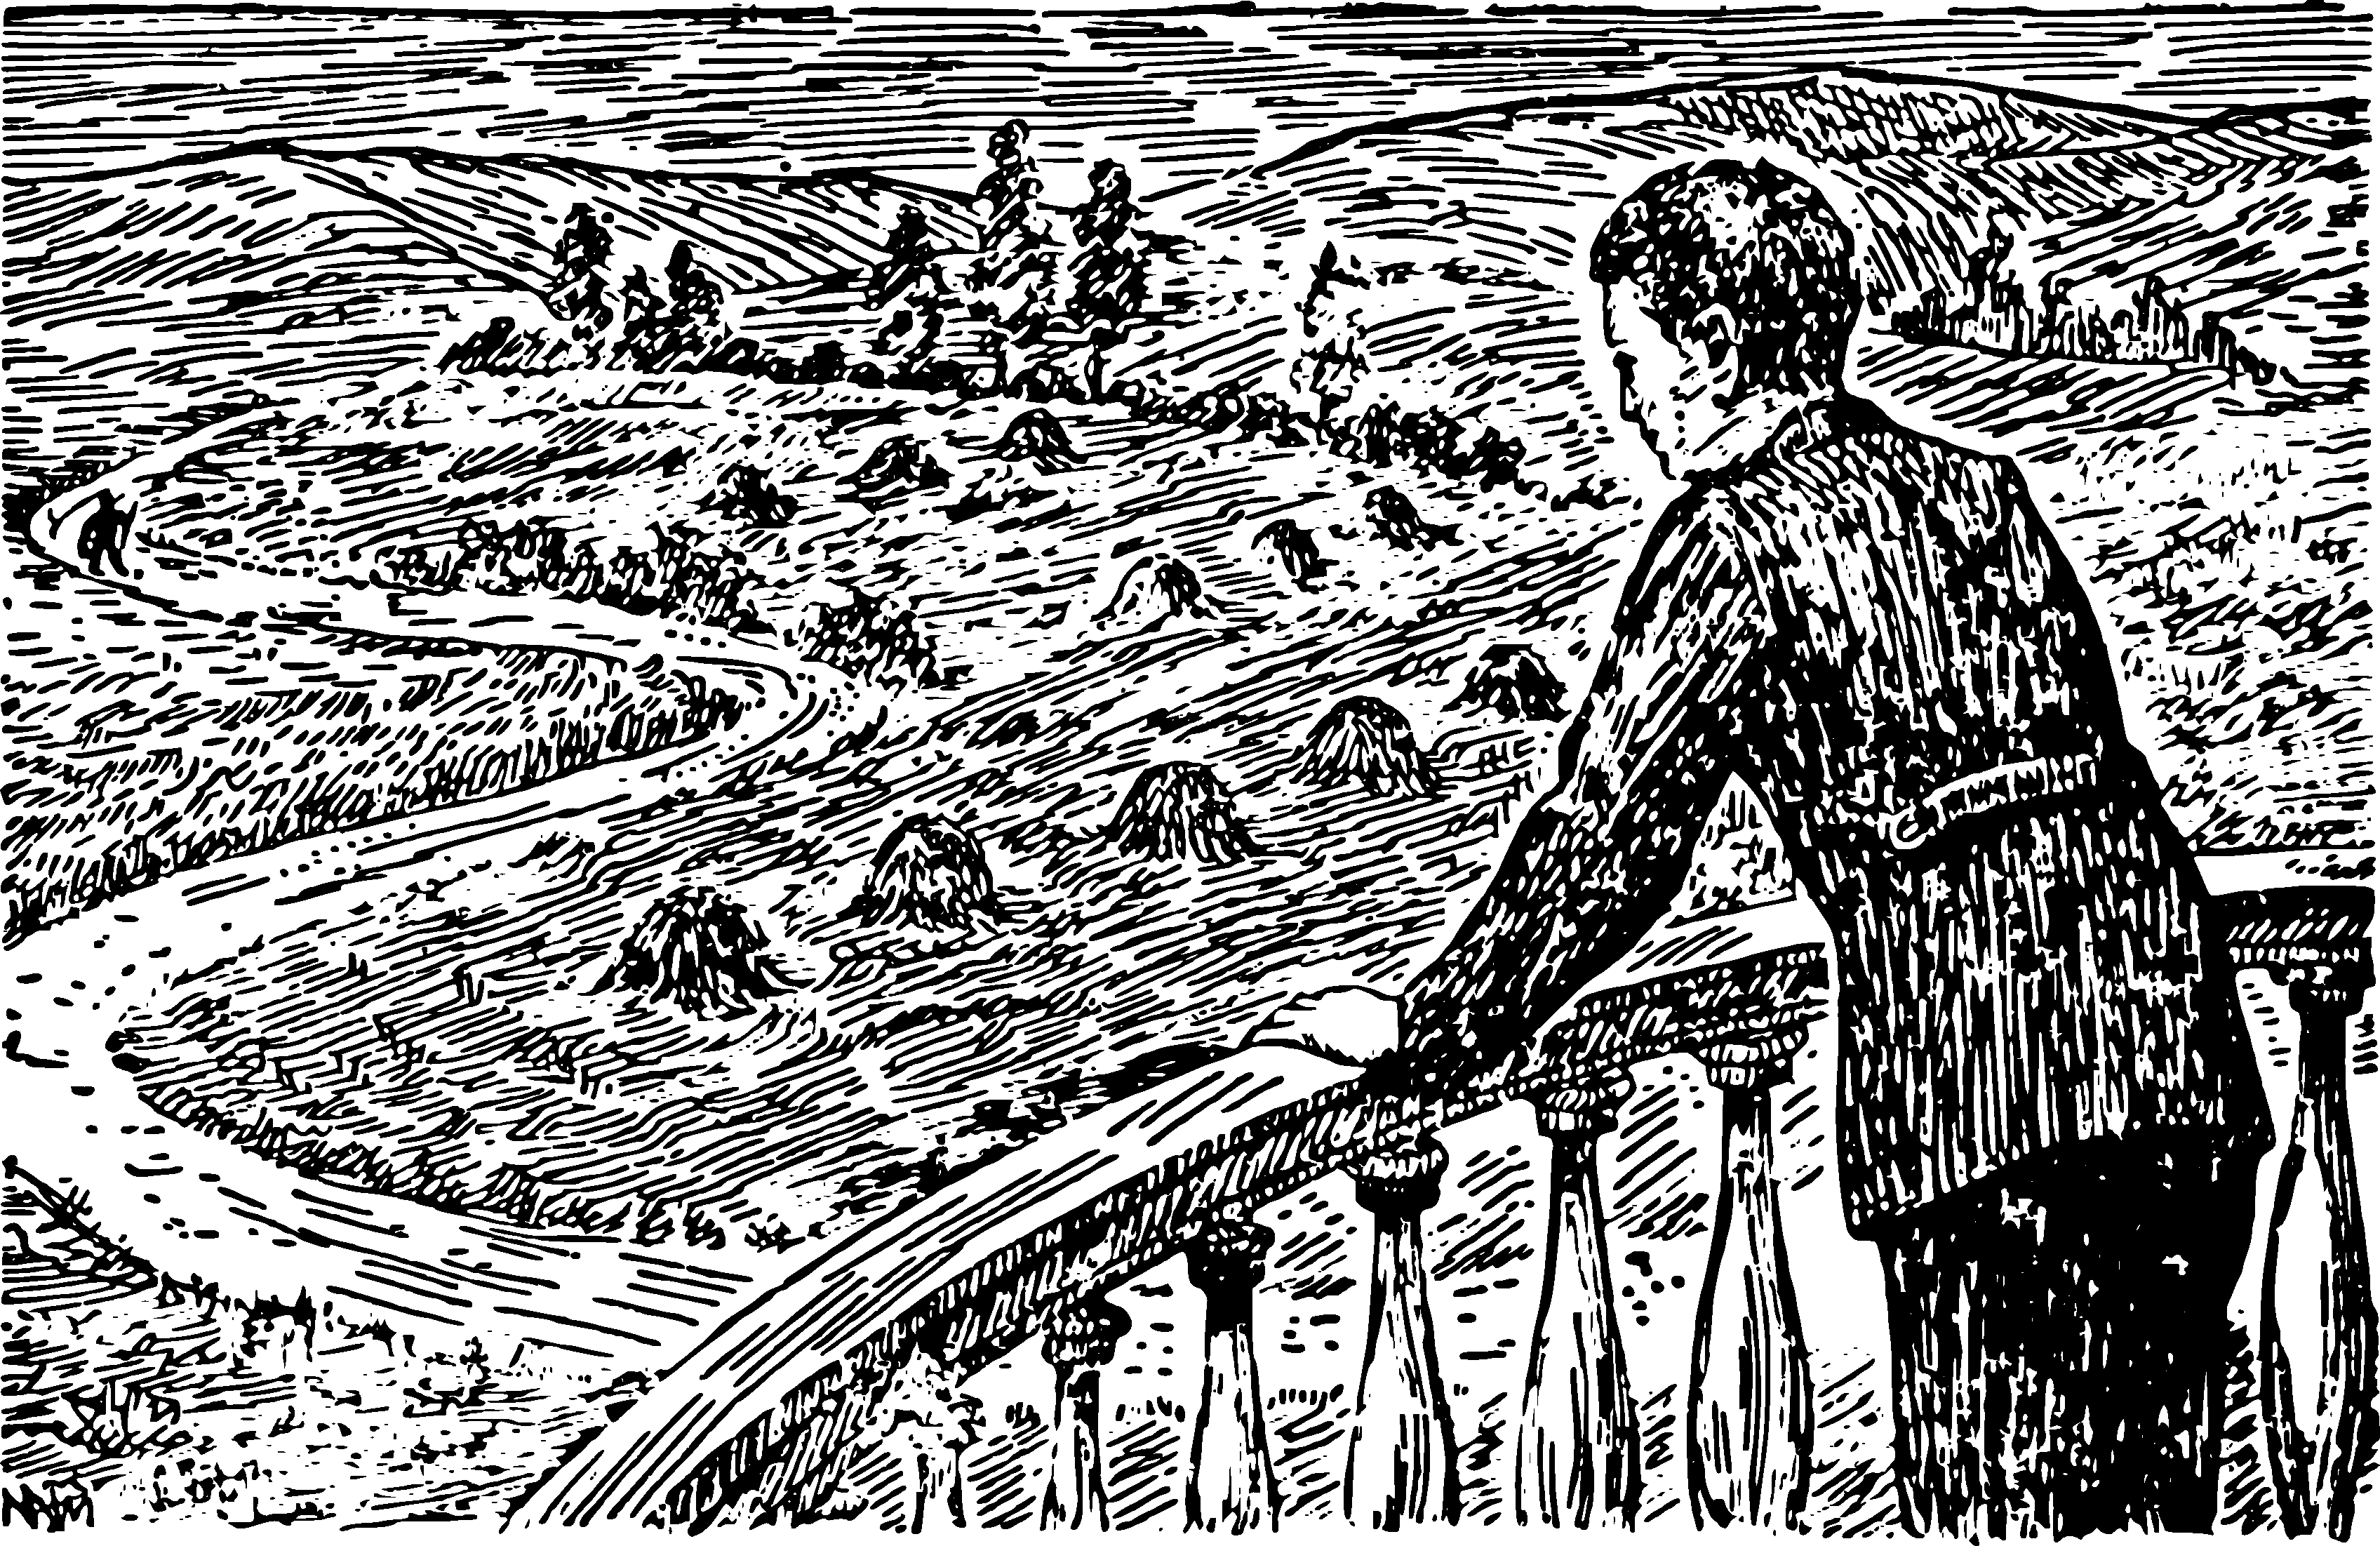
\includegraphics[width=0.9\textwidth]{figures/ch-03/fig-062.pdf}
\sidecaption{The human figure is visible from a distance of about hundred meters at an angle of \ang{1}.\label{fig-062}}
\end{figure}
So, a person appears at an angle of \ang{1} if they are approximately at a distance of 100 meters from us (\figr{fig-062}). If they move twice as far away -- to 200 meters -- they will be seen at an angle of half a degree; if they approach to a distance of 50 meters, the angle of view will increase to \ang{2}, and so on. It is also easy to calculate that a stick of 1 meter in length should appear to us at an angle of 1° at a distance of $360/(44/7) = \SI{57}{\meter}$.

At the same angle, we perceive an object of 1 cm from a distance of 57 cm, 1 km from a distance of 57 km, and so on -- in general, any object from a distance 57 times greater than its diameter. If we remember this number -- 57, we can quickly and easily perform all calculations related to the angular size of an object. For example, if we want to determine how far we need to move an apple with a diameter of 9 cm to see it at an angle of \ang{1}, it is sufficient to multiply 9 by 57 -- we get 513 cm, or about 5 meters; from twice the distance, it is perceived at half the angle -- half a degree, i.e., it appears the size of the Moon.

In the same way, for any object, we can calculate the distance at which it appears to be the same size as the lunar disk.

\section{Plate and Moon} 
\label{sec-3.3}

\ques At what distance should a plate with a diameter of 25 cm be moved away to appear the same size as the Moon in the sky?

\ans $\SI{25}{\centi\meter} \times 57 \times 2 = \SI{2850}{\centi\meter} = \SI{28}{\meter}$.

\section{Moon and Copper Coins} 
\label{sec-3.4}

\ques Perform the same calculation for a five-kopeck coin (diameter 25 mm) and a three-kopeck coin (22 mm).

\ans For the five-kopeck coin: \(0.025 \text{ m} \times 57 \times 2 = 2.85 \text{ meters}\),
For the three-kopeck coin: \(0.022 \text{ m} \times 57 \times 2 = 2.514 \text{ meters}\).

If it seems unbelievable to you that the Moon appears no larger than a two-kopeck coin from a distance of four steps or an ordinary pencil from a distance of 80 cm, -- hold the pencil at arm's length against the full Moon disk: it will easily cover it. Strangely enough, the most suitable comparison object for the Moon in terms of perceived size is not a plate, not an apple, not even a cherry, but a pea or, even better, a match head! Comparing it to a plate or an apple implies moving them to an unusually large distance; we see an apple in our hands or a plate on the dining table ten to twenty times larger than the lunar disk. And only a match head, which we examine at a distance of 25 cm from the eye (`distance of distinct vision'), is seen at an angle of half a degree, i.e., the same size as the Moon.

The fact that the lunar disk deceptively appears to grow in the eyes of most people by 10 to 20 times is one of the most curious optical illusions. It depends, one might think, mostly on the \emph{brightness} of the Moon: the full moon stands out against the sky much more sharply than plates, apples, coins, and other comparison objects do amidst the surrounding environment.\sidenote{For the same reason, the incandescent filament of an electric light bulb seems to us much thicker than in a cold, non-luminous state.}

This illusion is imposed on us with such irresistible force that even artists, distinguished by a keen eye, succumb to it alongside others and depict the full moon in their paintings much larger than it should be. It is enough to compare the landscape painted by an artist with a photograph to be convinced of this.

The same applies to the Sun, which we see from Earth at the same angle of half a degree; although the true diameter of the solar sphere is 400 times larger than that of the lunar one, its distance from us is also 400 times greater.


\section{Sensational Photographs}
\label{sec-3.5}

To explain the important concept of the angle of view, let's deviate a bit from our main topic — geometry in open fields — and provide a few examples from the realm of photography.

On the movie screen, you've surely seen such catastrophes as train collisions or such incredible scenes as a car driving on water.

Recall the movie `Captain Grant's Children.' What a strong impression -- isn't it? -- the scenes of the shipwreck during the storm or the sight of crocodiles surrounding the boy stuck in the swamp left on you. Of course, no one thinks that such photographs were taken directly from real life. But how were they obtained?
\begin{figure}[h!]
\centering
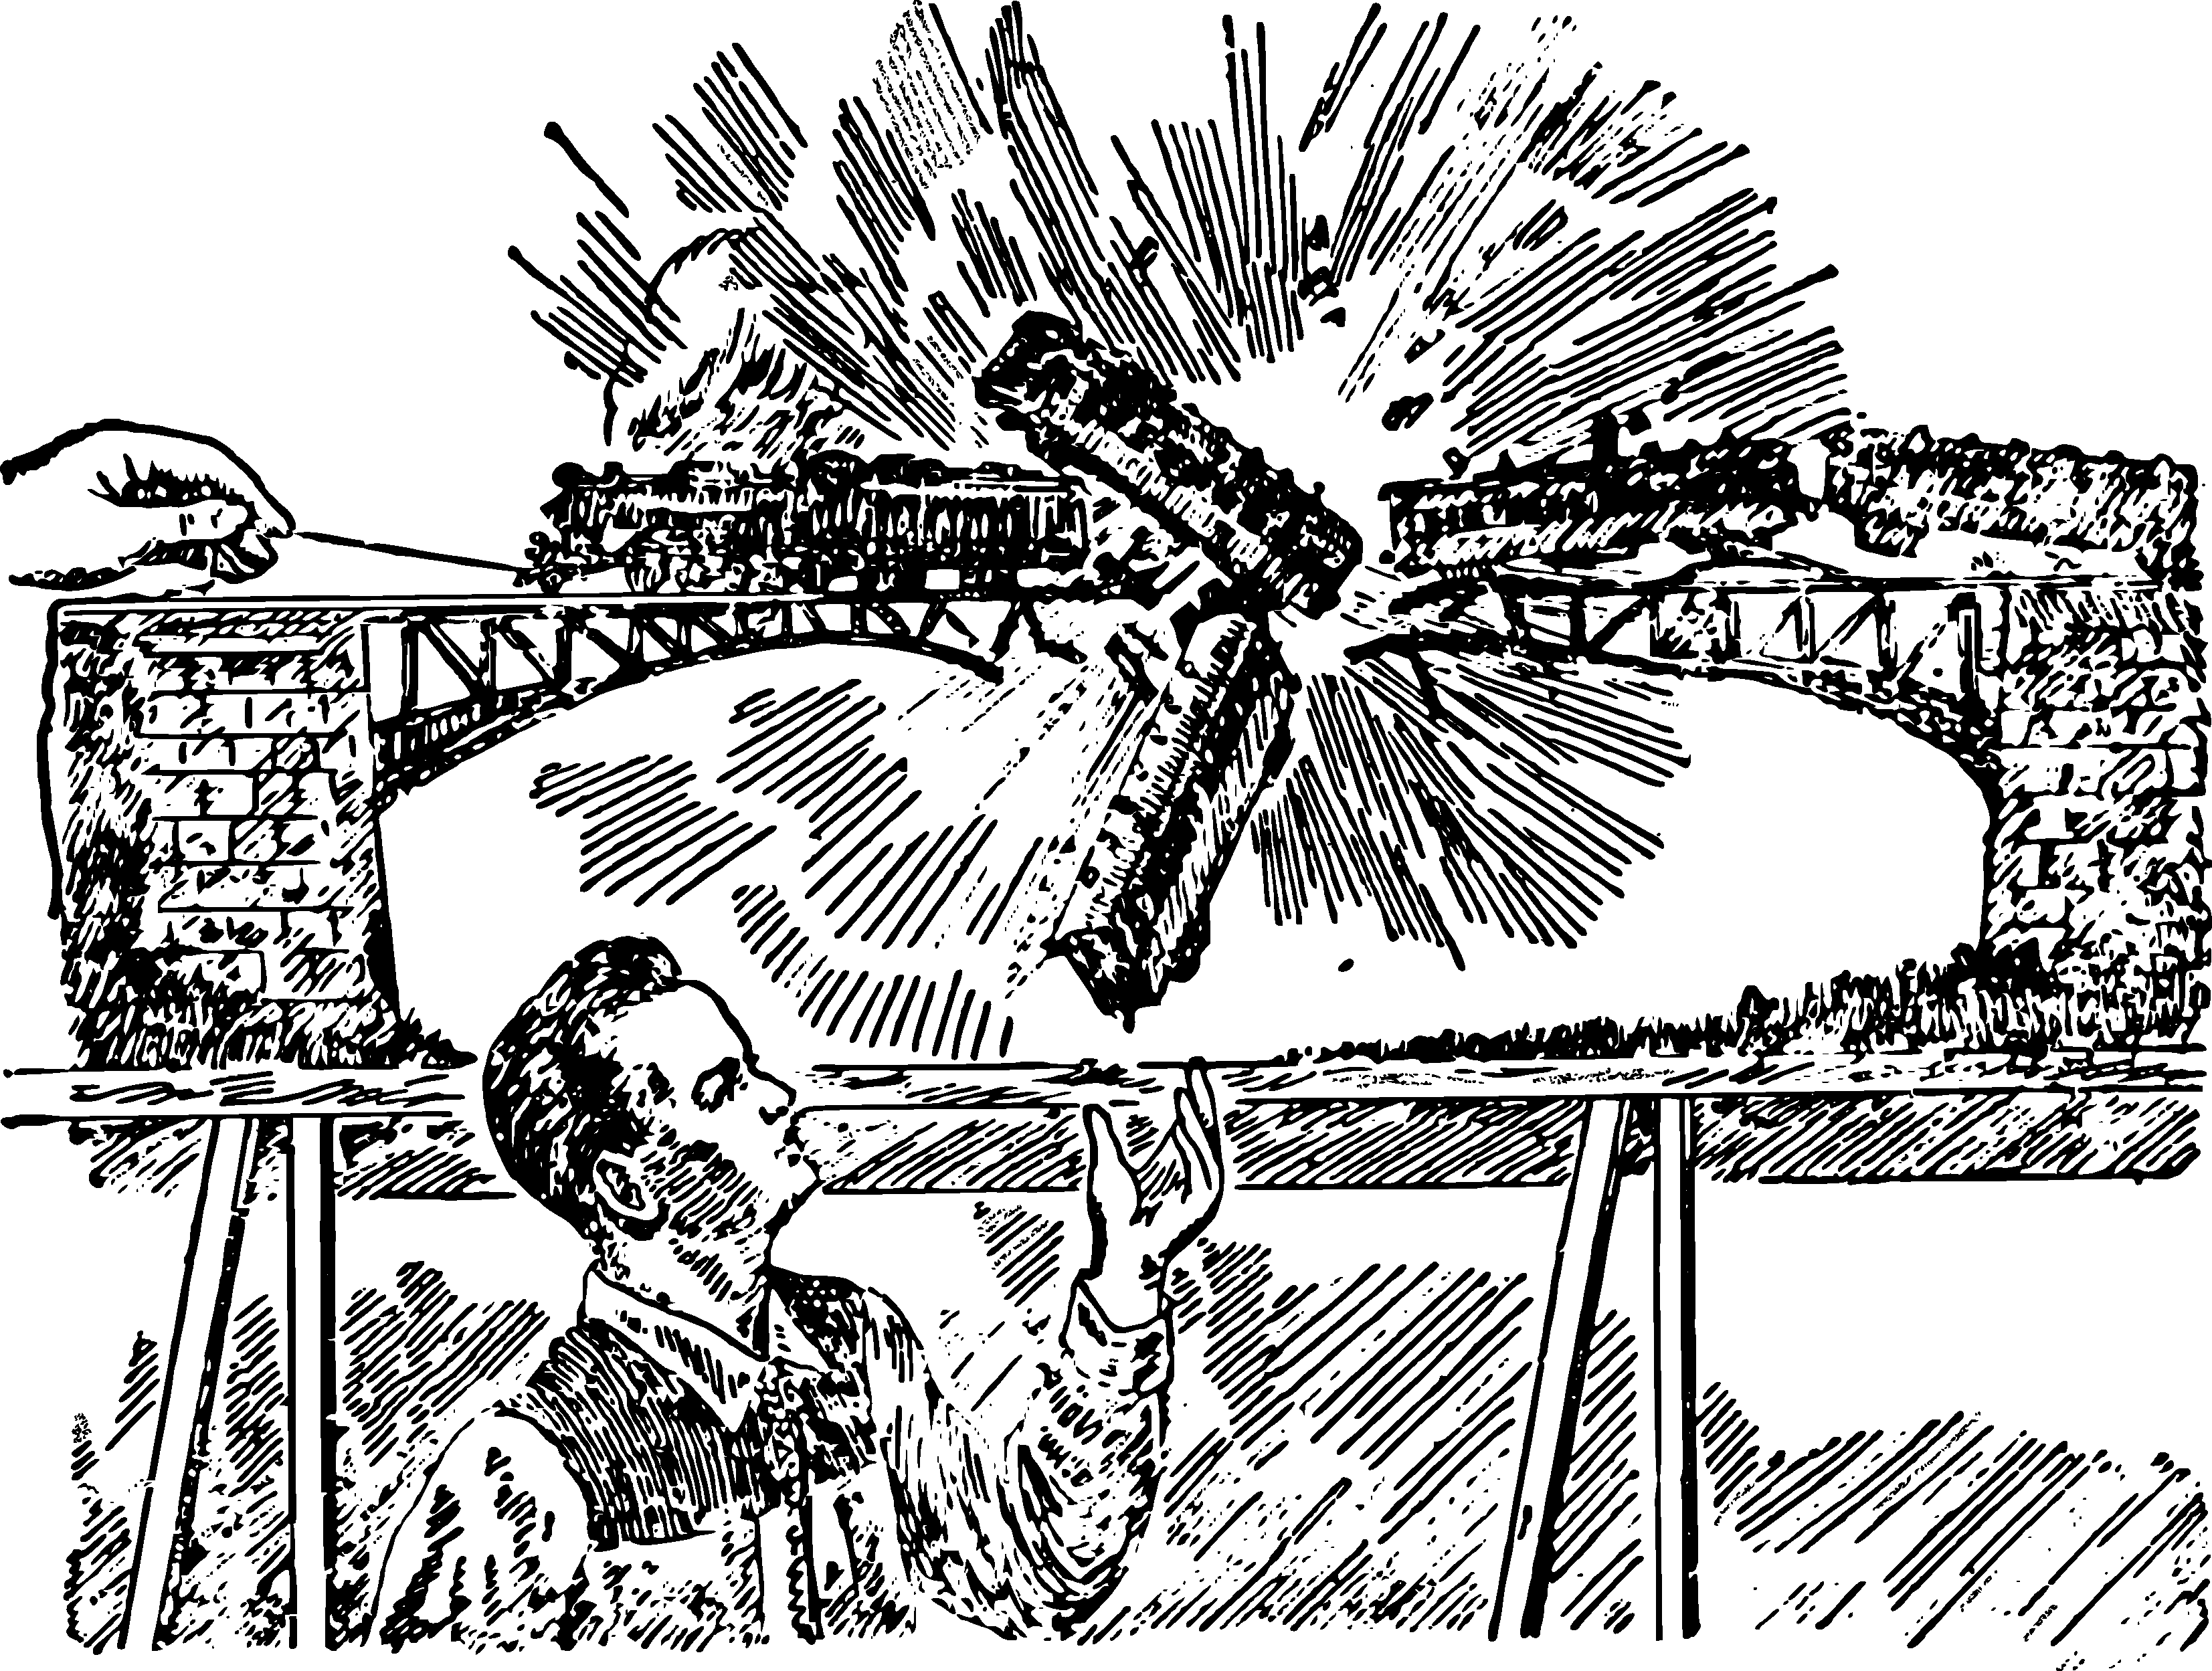
\includegraphics[width=0.9\textwidth]{figures/ch-03/fig-063.pdf}
\sidecaption{Preparing a train accident for filming.\label{fig-063}}
\end{figure}


The secret is revealed by the illustrations attached here. In \figr{fig-063}, you see the `catastrophe' of a toy train in a toy setting; in \figr{fig-064} -- a toy car being pulled on a string behind an aquarium. This is the `nature' from which the film was shot. But why do we succumb to the illusion when we see these images on the screen, as if we were looking at real trains and cars? After all, here, in the illustrations, we would immediately notice their miniature size, even if we couldn't compare them with the size of other objects. The reason is simple: toy trains and cars are filmed for the screen from a very close distance; therefore, they appear to the viewer at approximately the same angle of view as we usually see real trains and cars. That's the whole secret of the illusion.

\begin{figure}[h!]
\centering
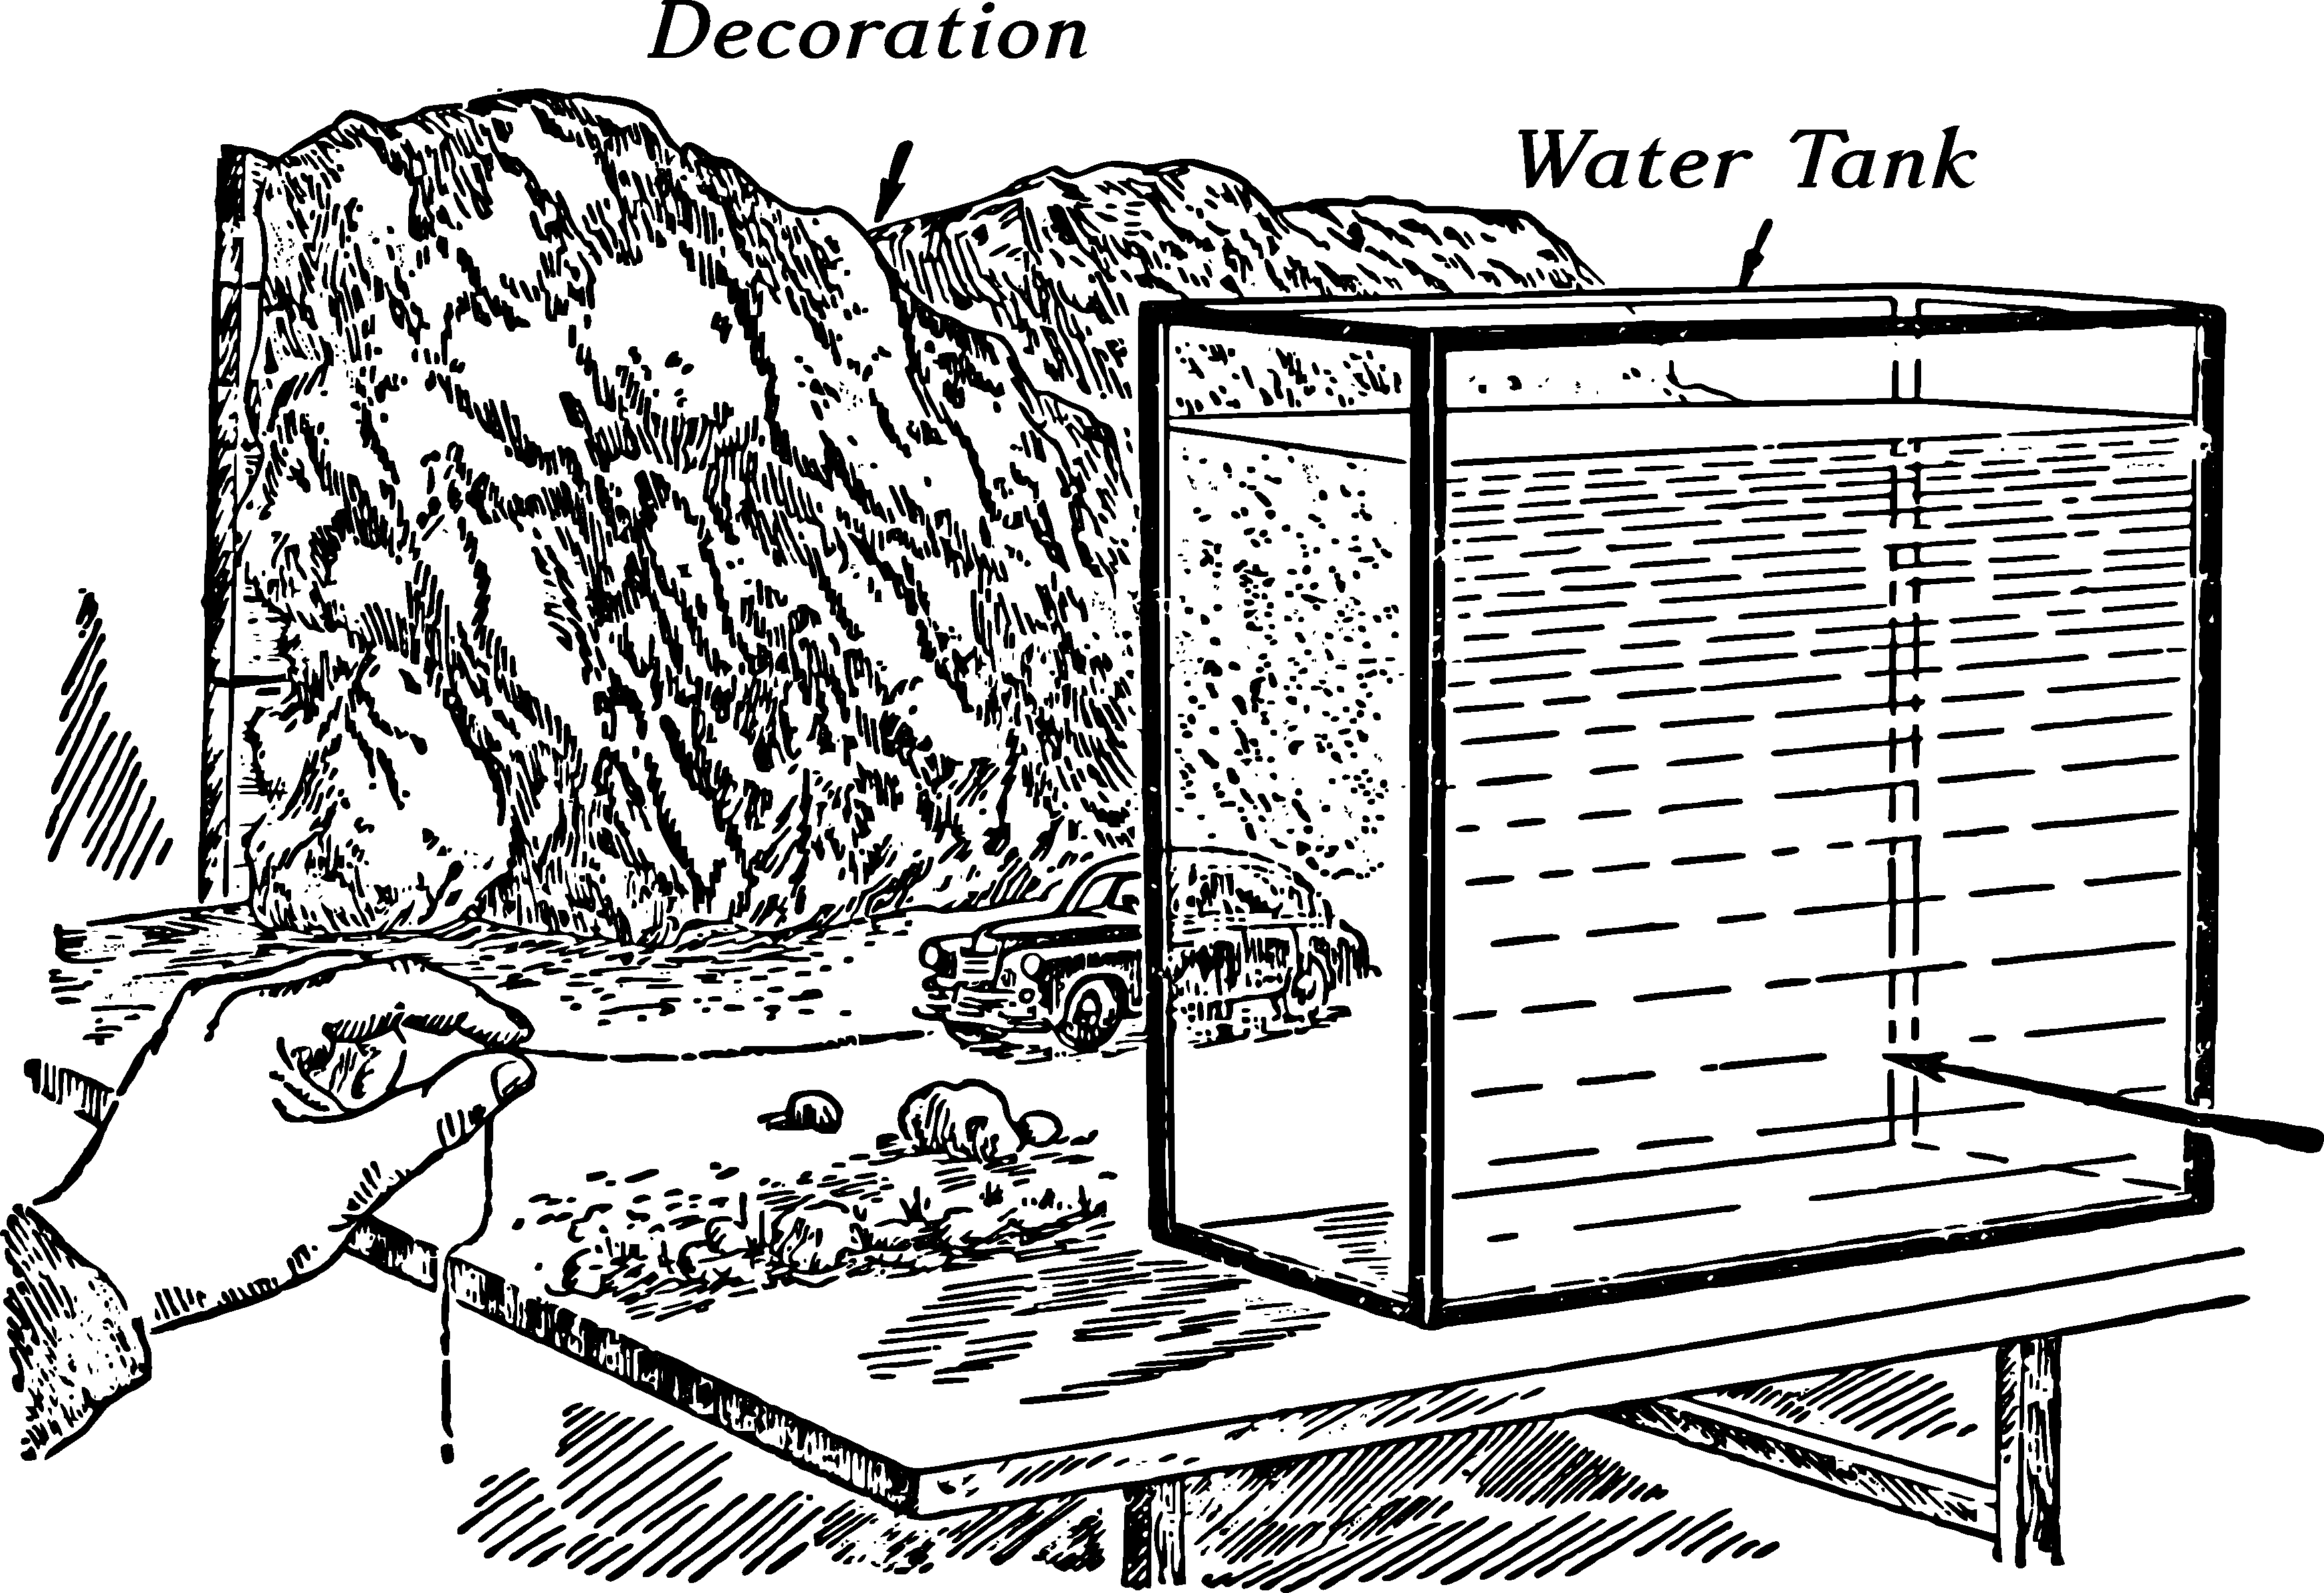
\includegraphics[width=0.9\textwidth]{figures/ch-03/fig-064.pdf}
\sidecaption{The underwater road trip.\label{fig-064}}
\end{figure}

Or here's another frame from the movie `Ruslan and Ludmila' (\figr{fig-065}). A huge head and a small Ruslan on a horse. The head is placed on a model field close to the camera. And Ruslan on the horse -- at a considerable distance. That's the entire secret of the illusion.

\begin{figure}[h!]
\centering
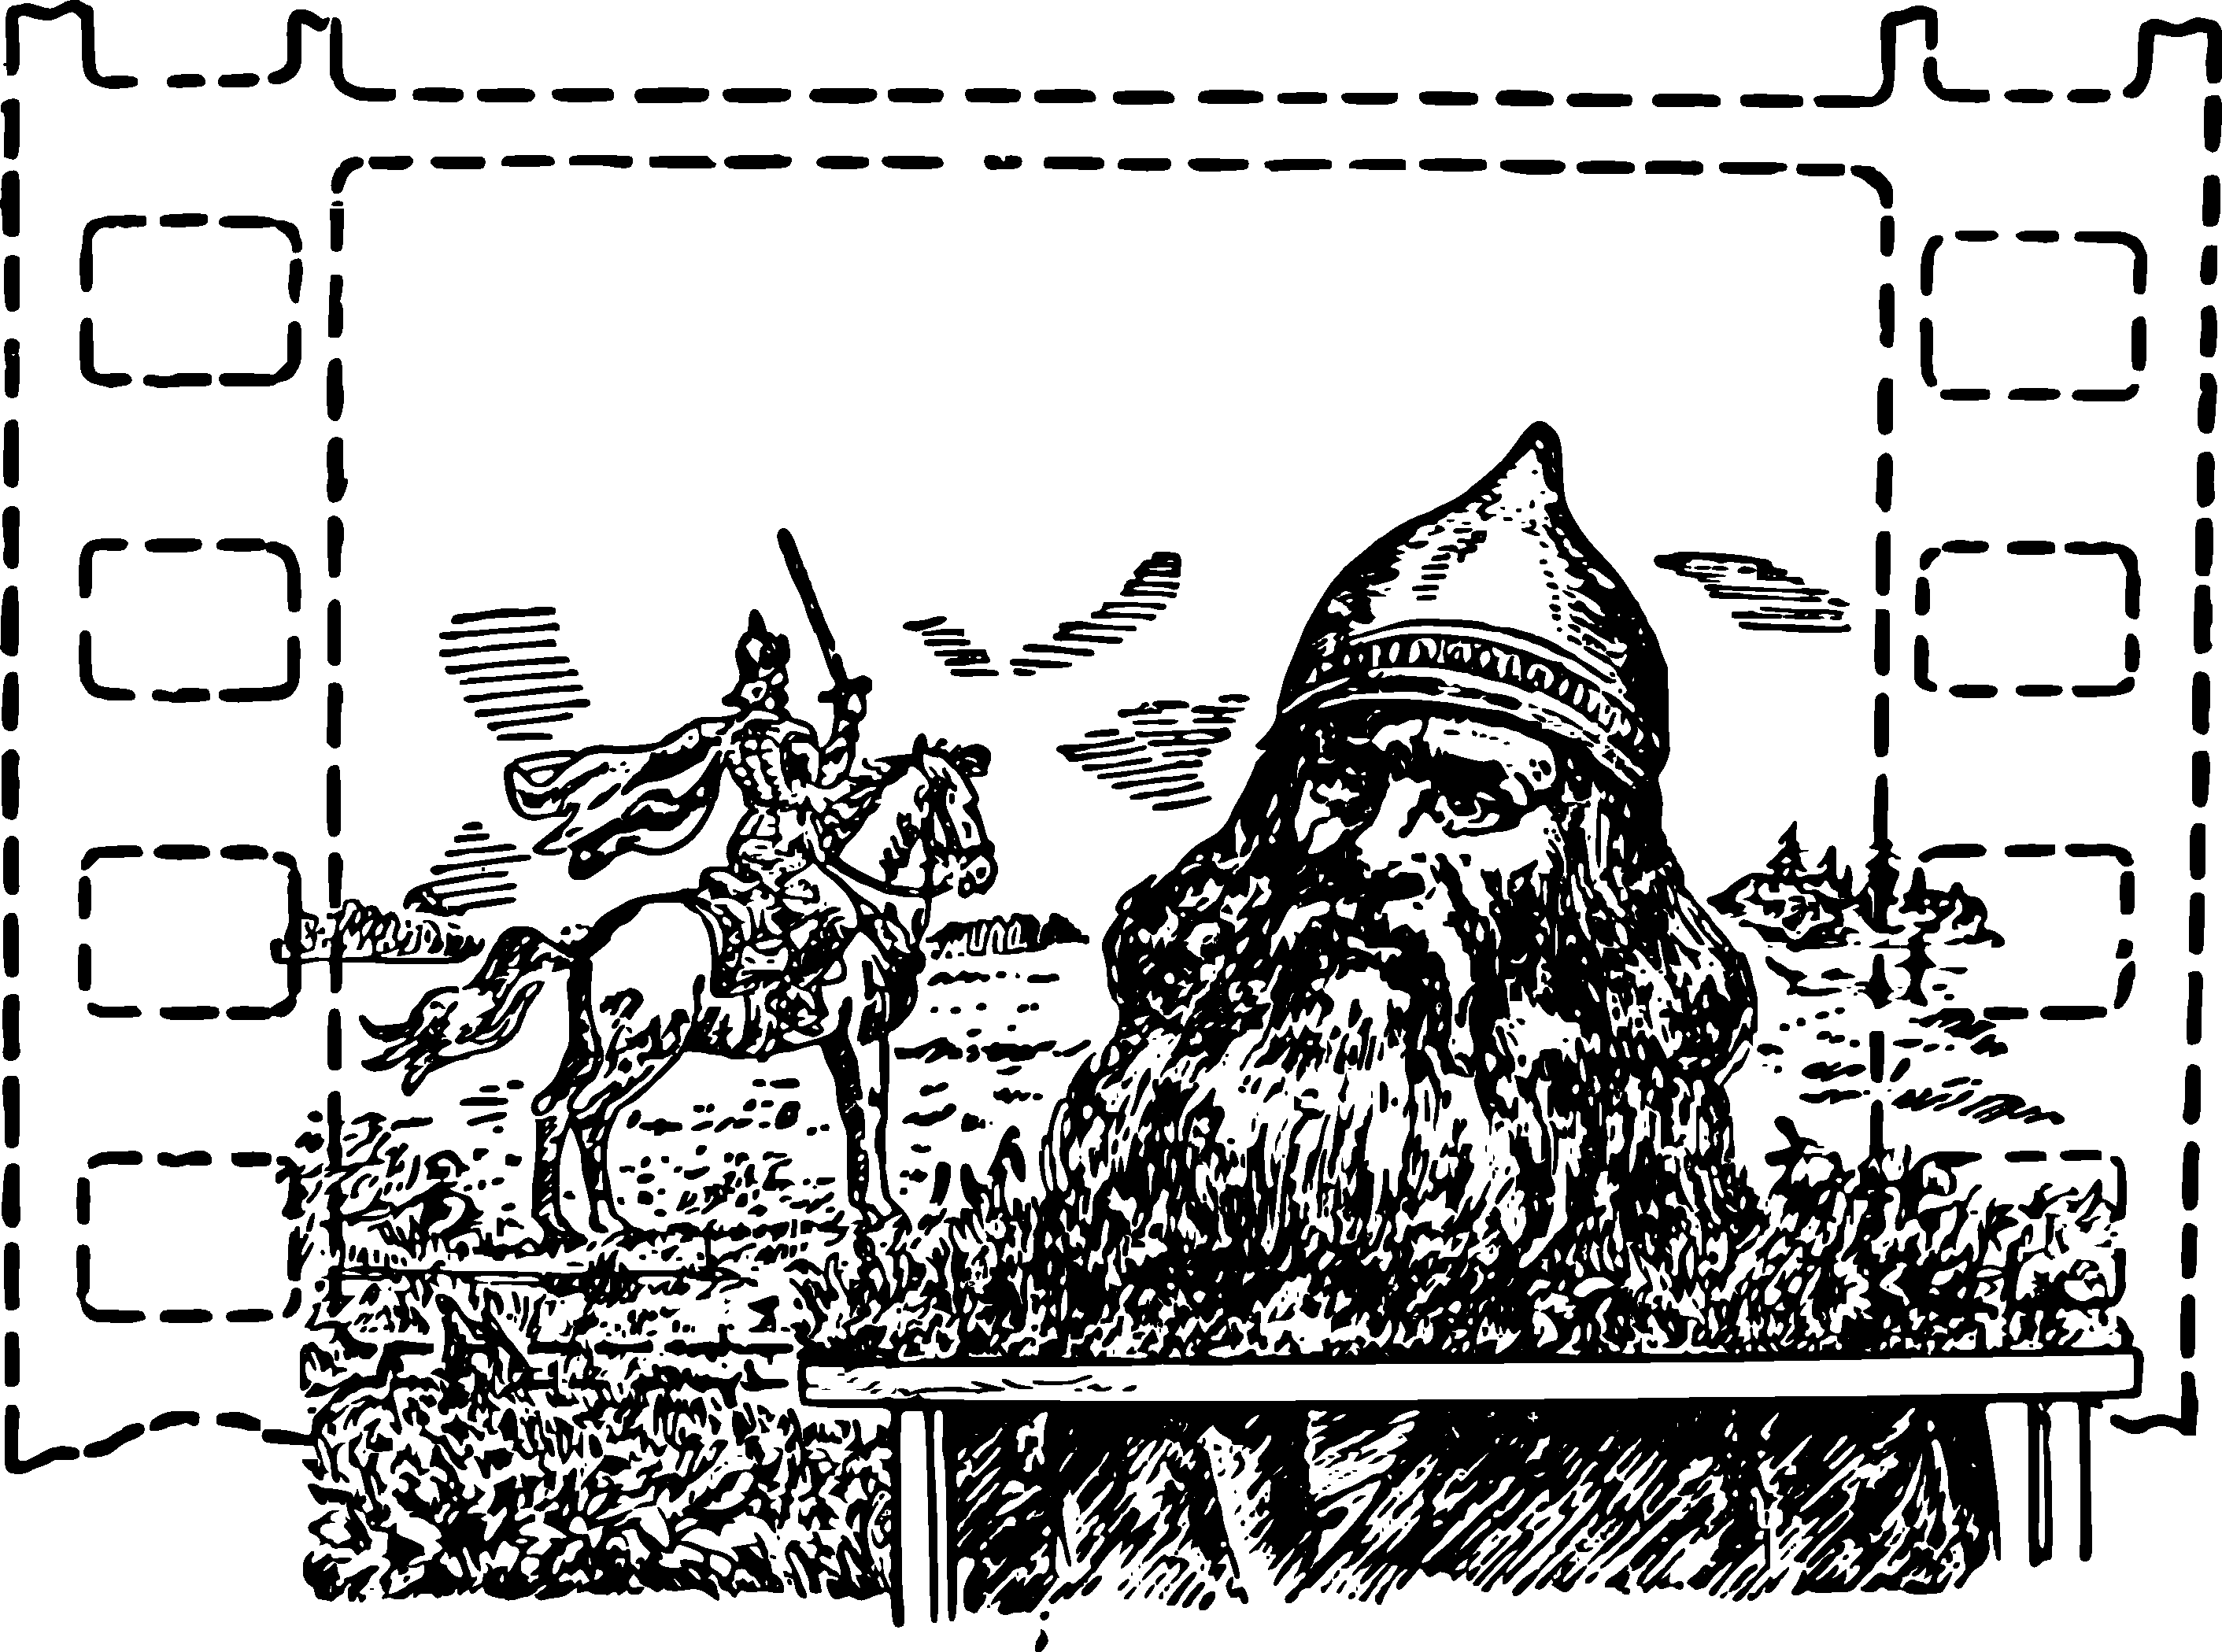
\includegraphics[width=0.9\textwidth]{figures/ch-03/fig-065.pdf}
\sidecaption{A shot from the movie \emph{Ruslan and Lyudmila}.\label{fig-065}}
\end{figure}

\section{Reservoir Set Decoration}
\label{sec-3.6}

\figr{fig-066} is another example of an illusion based on the same principle. You see a strange landscape reminiscent of the nature of ancient geological epochs: bizarre trees resembling giant mosses, on them -- huge water drops, and in the foreground -- a gigantic monster resembling harmless frogs. Despite such an unusual view, the drawing is made with subtlety: it's nothing but a small patch of soil in the forest, only drawn from an unusual angle of view. We never see moss stems, water drops, frogs, etc., at such a large angle of view, and therefore the drawing seems so alien, unfamiliar to us. Before us is a landscape as we would see it if we were shrunk to the size of an ant. 

\begin{marginfigure}[-1cm]%[h!]
\centering
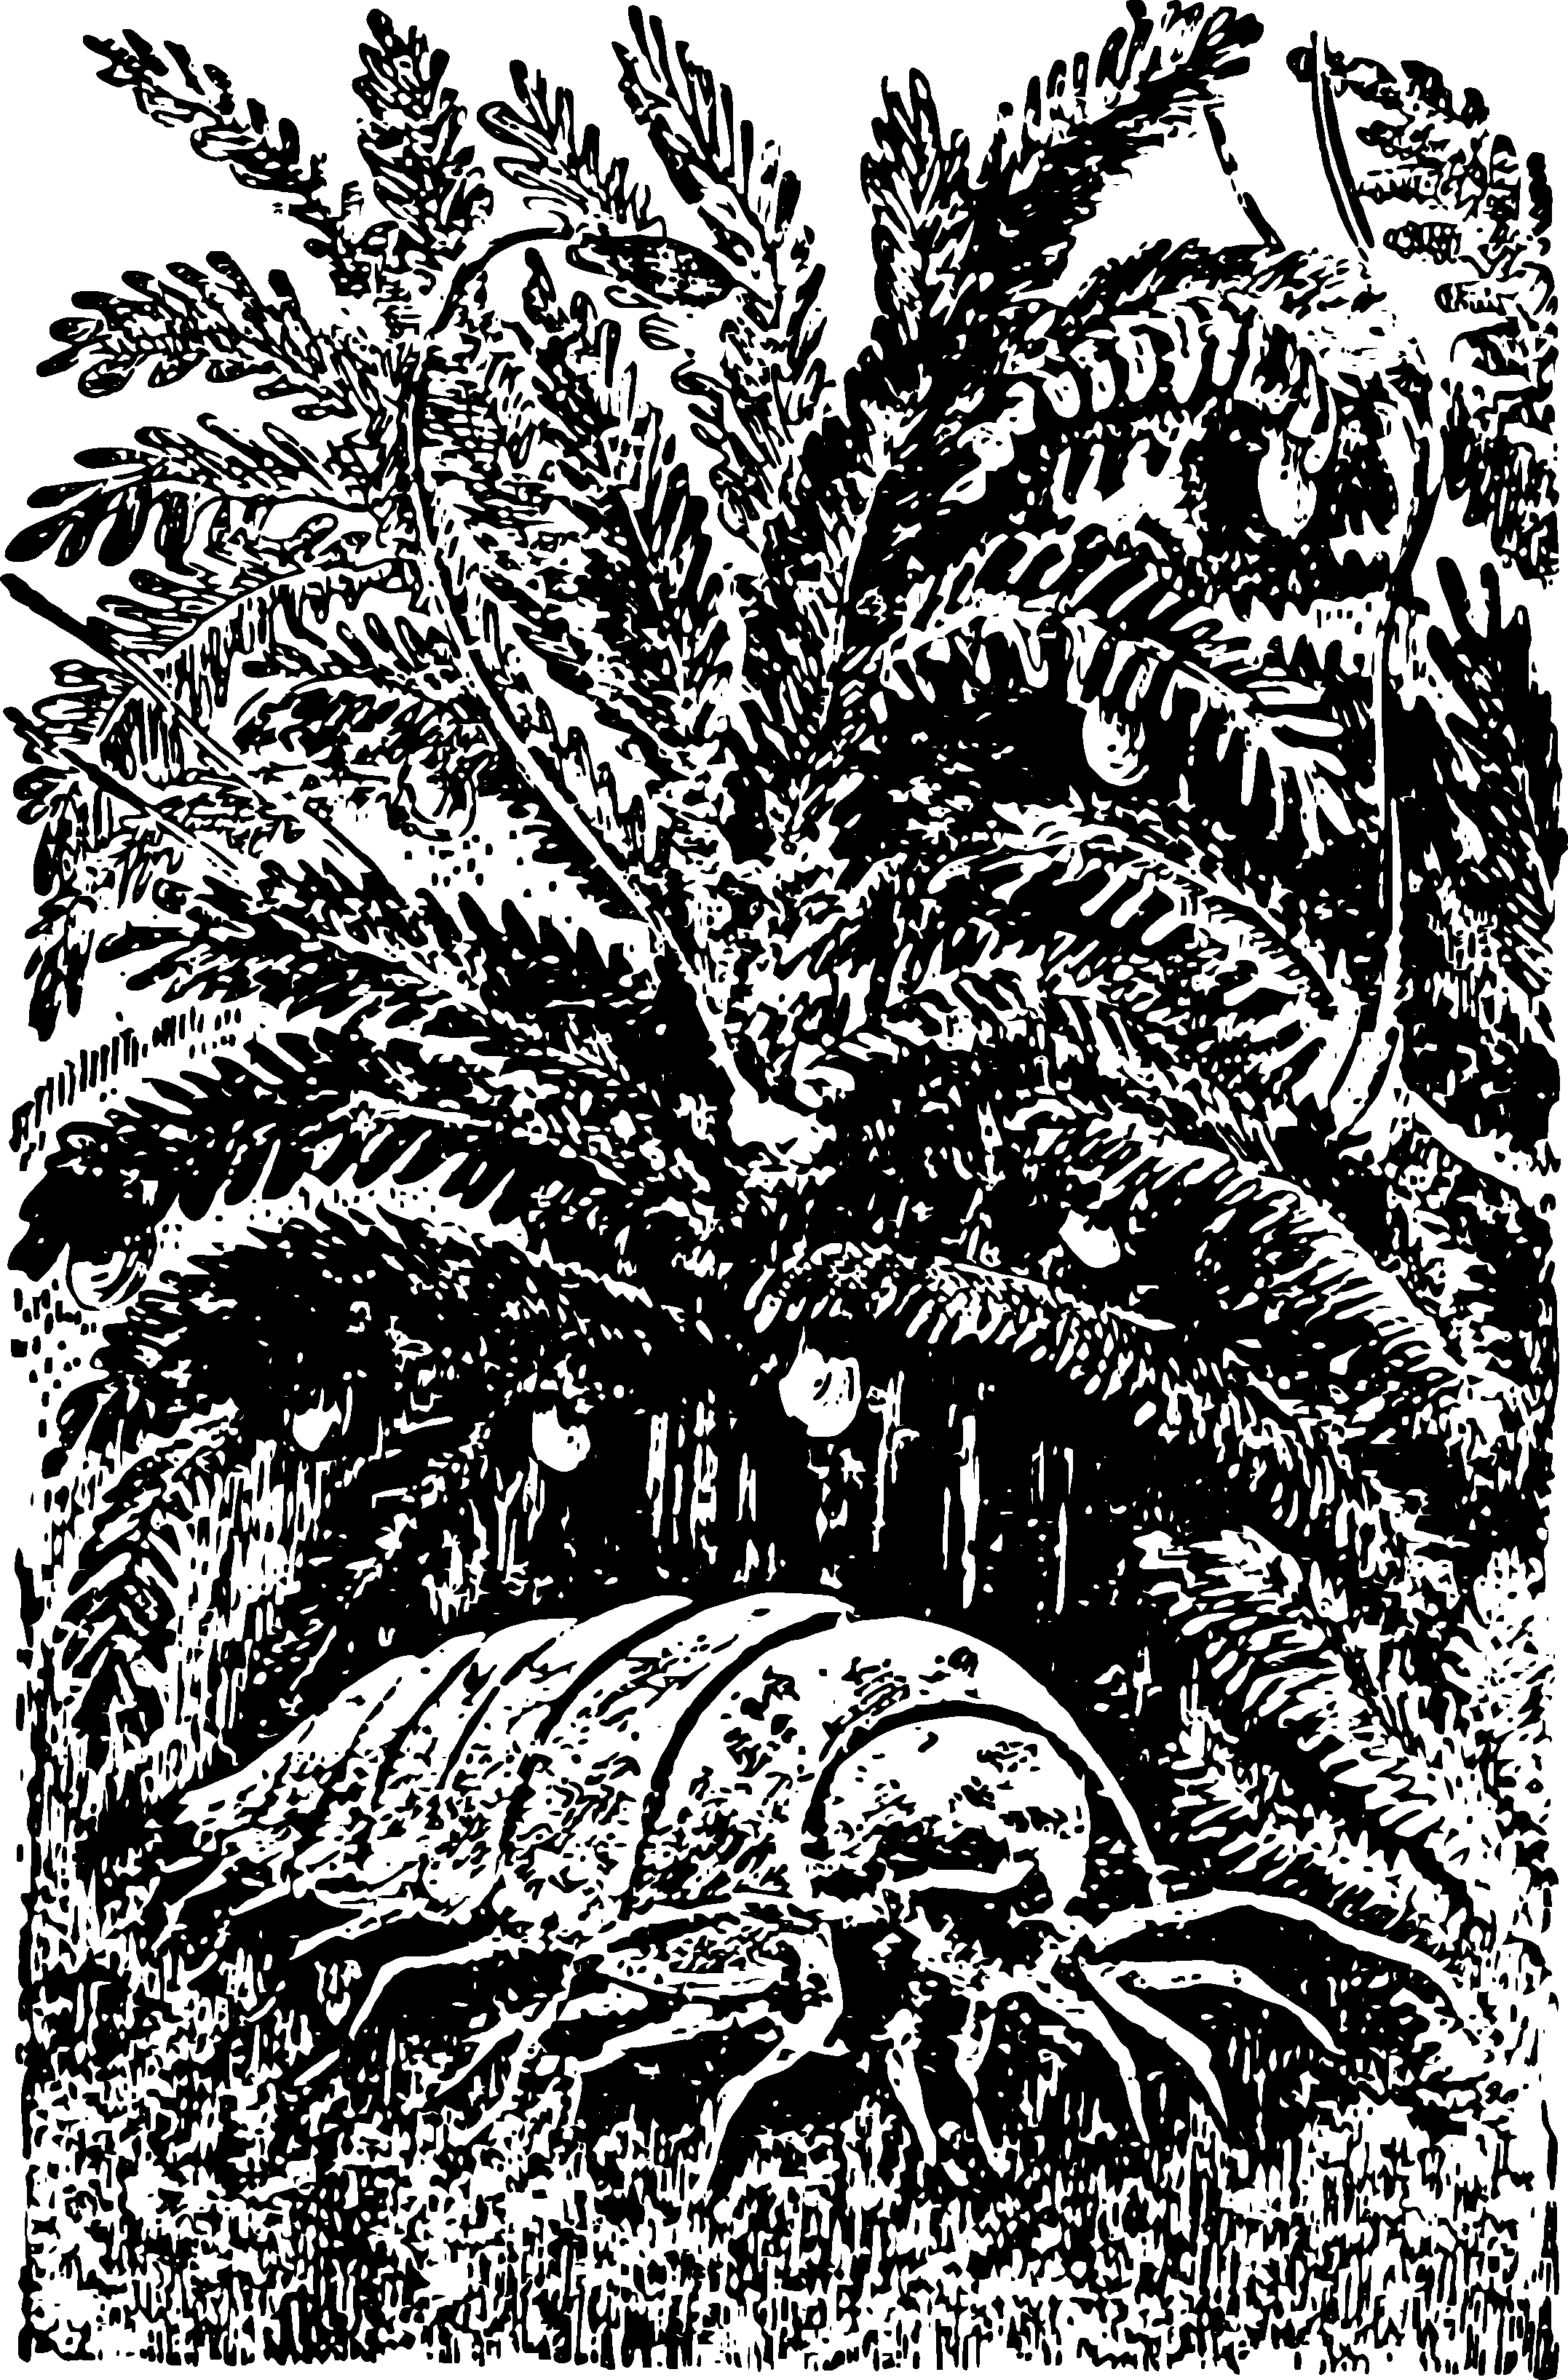
\includegraphics[width=\textwidth]{figures/ch-03/fig-066.pdf}
\sidecaption{Mysterious landscape depicted from nature.\label{fig-066}}
\end{marginfigure}

Swindlers from bourgeois newspapers act in the same way to create fake reportage photographs. One foreign newspaper once published a note criticising the city administration for allowing huge snow mountains to form on the city streets. To support this, an impressive photo of one such mountain was provided (\figr{fig-067}, left). Upon examination, it turned out that the nature for the photograph was a small snowdrift, taken by the `joker' photographer from a very close distance, i.e., at an unusually large angle of view (\figr{fig-067}, right). 

\begin{figure}[h!]
\centering
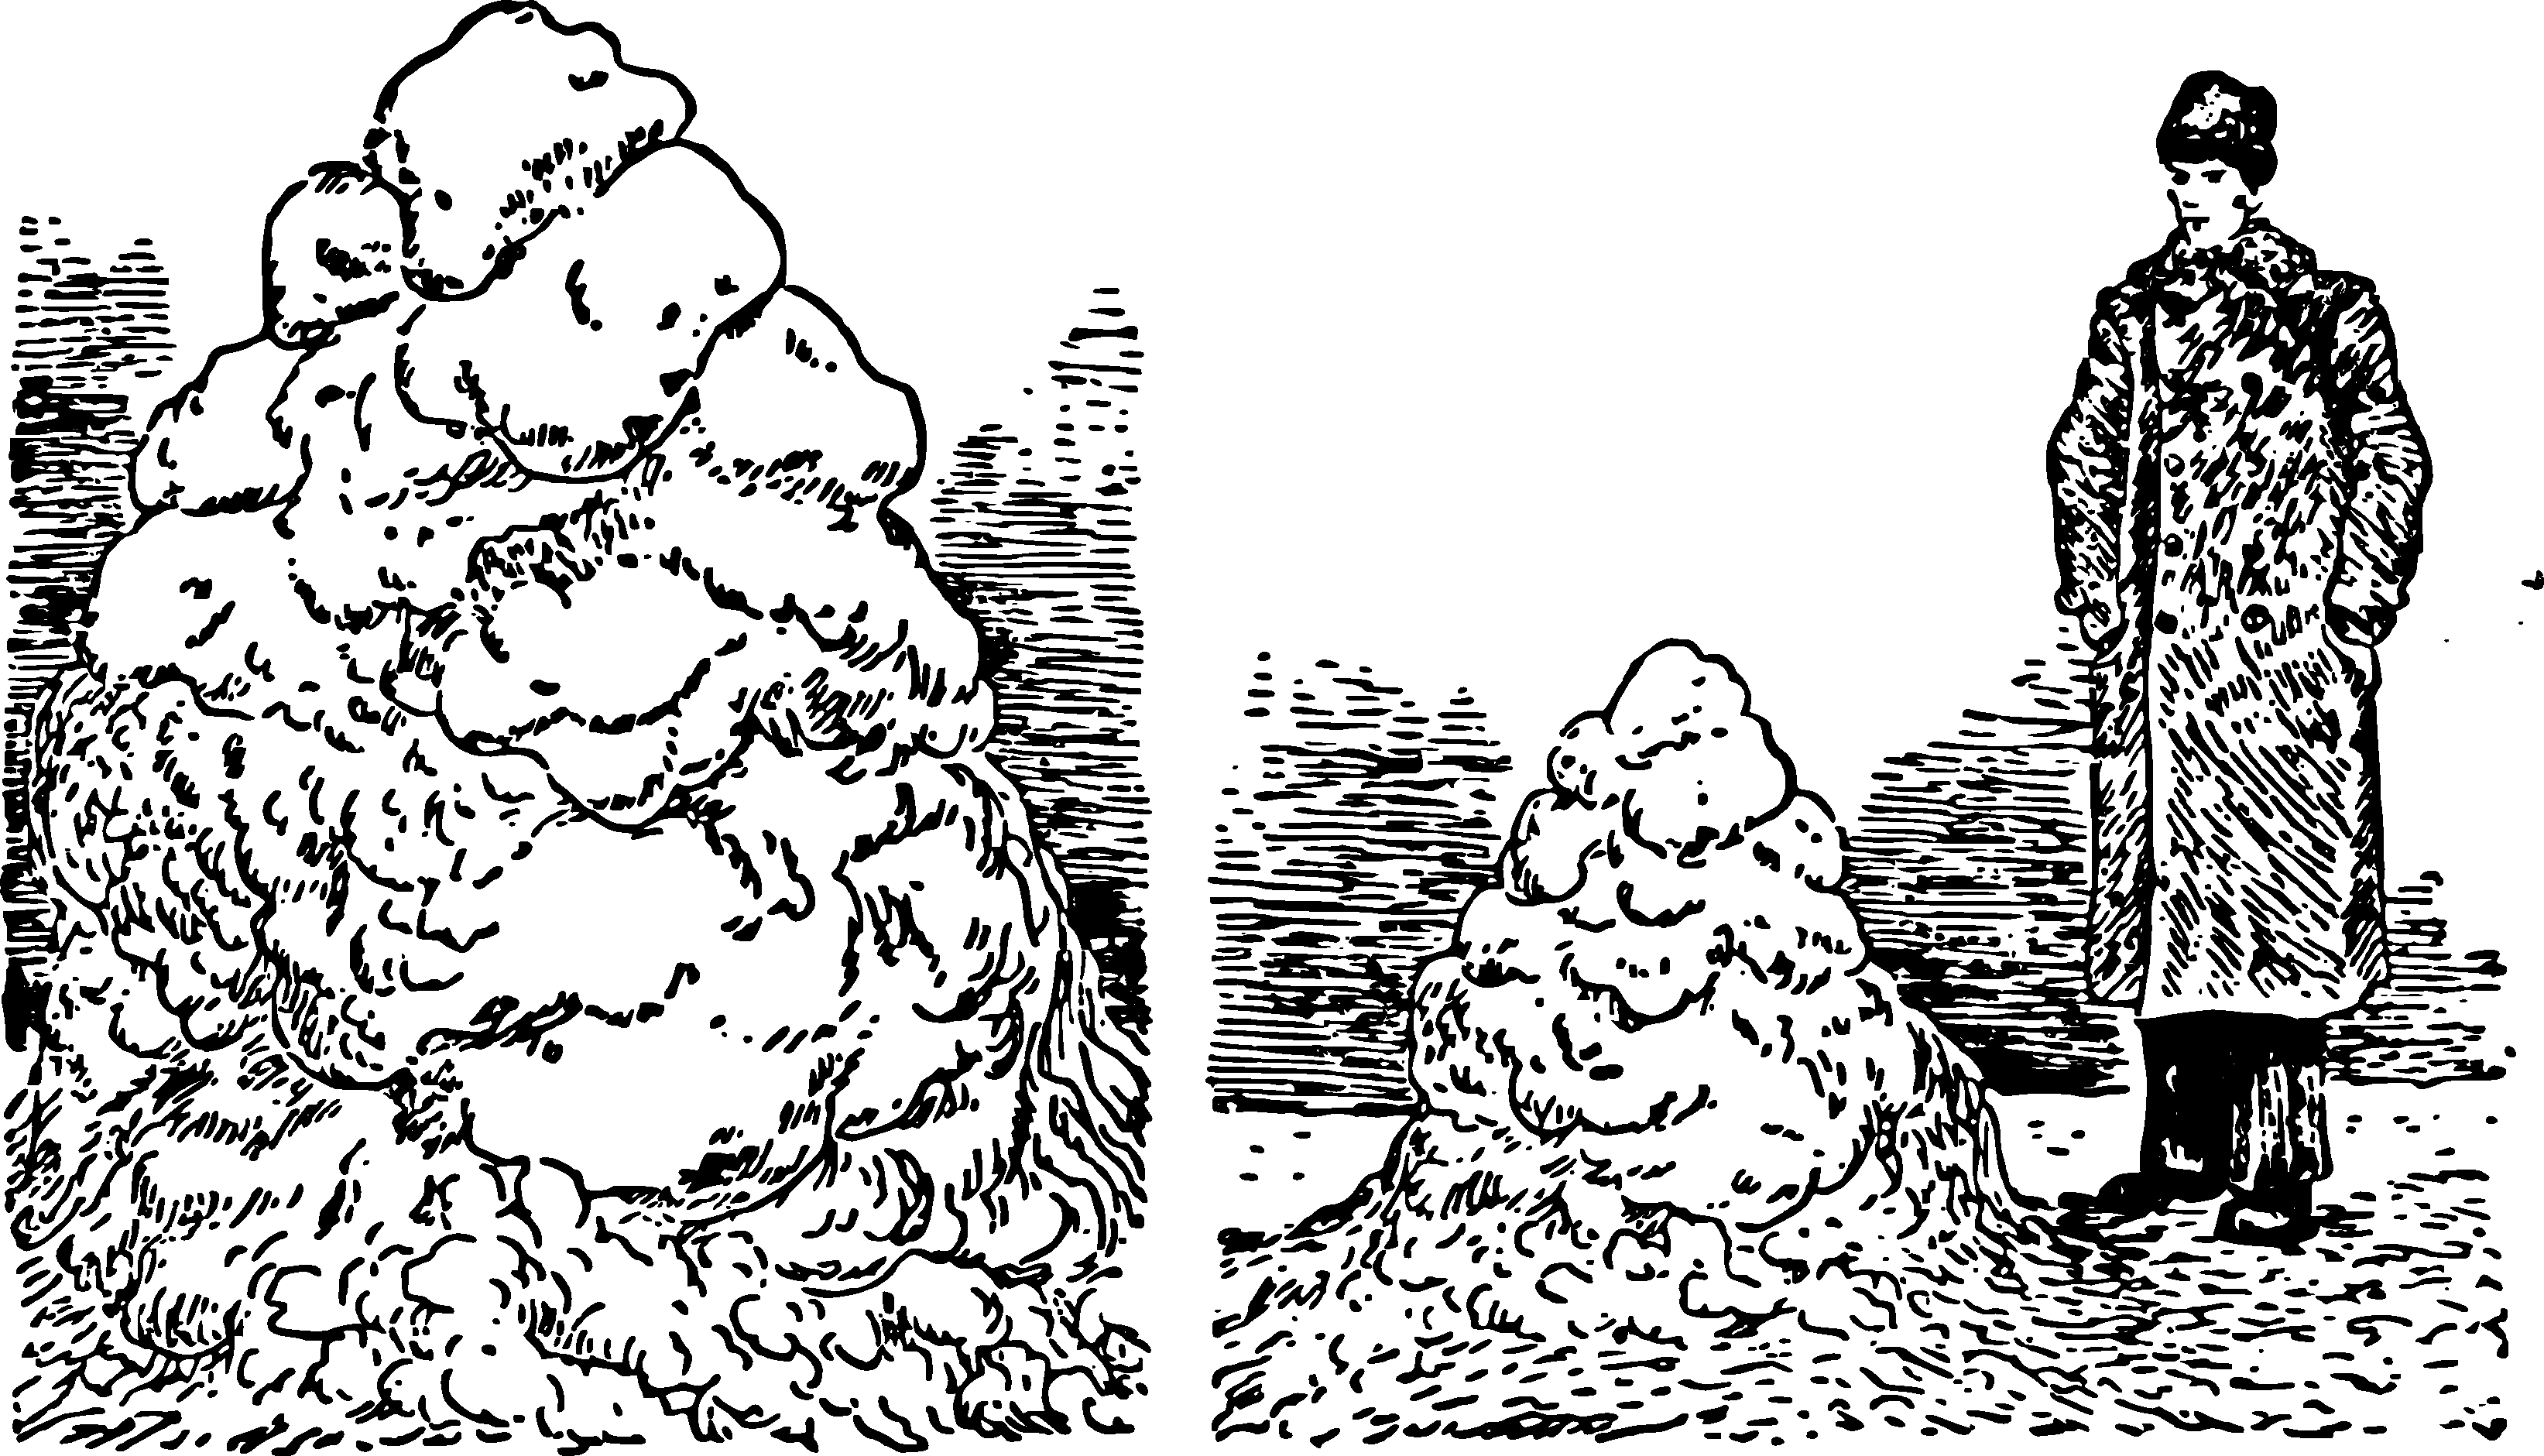
\includegraphics[width=\textwidth]{figures/ch-03/fig-067.pdf}
\sidecaption{Snow mountain in a photograph (left) and in nature (right).\label{fig-067}}
\end{figure}

Another time, the same newspaper reproduced a photo of a wide crevice in the rock near the city; it served, according to the newspaper, as the entrance to an extensive underground cave, where a group of careless tourists who dared to enter the cave for exploration disappeared without a trace. A volunteer search party equipped to search for the lost discovered that the crevice was photographed\dots{} from a barely noticeable crack in the icy wall, a centimetre wide!



\section{Living Protractor}
\label{sec-3.7}

Making a simple protractor device yourself is not very difficult, especially if you use a protractor. But sometimes even a homemade protractor may not be at hand during a countryside walk. In such cases, you can rely on the services of a ``living protractor'' that is always with us. These are our own fingers. To use them for a rough estimate of viewing angles, you just need to make a few preliminary measurements and calculations.

First of all, you need to determine at what angle we see the fingernail of our outstretched index finger. The usual width of a nail is \SI{1}{\centi\meter}, and its distance from the eye in such a position is about \SI{60}{\centi\meter}; therefore, we see it at an angle of about \ang{1} (slightly less because an angle of \ang{1} would be at a distance of \SI{57}{\centi\meter}). For teenagers, the nail is smaller, but the arm is shorter, so the viewing angle for them is approximately the same -- \ang{15}. The reader would do well to perform this measurement and calculation for themselves, relying on book data, to make sure the result is not too far from \ang{15}; if the deviation is significant, you should try another finger.

Knowing this, you have a way to estimate small viewing angles literally with your bare hands. Each distant object, which is just covered by the fingernail of your outstretched index finger, is seen by you at an angle of \ang{1} and, therefore, is 57 times farther away than its width. If the nail covers half of the object, it means its angular size is \ang{2}, and the distance is equal to 28 widths.

The Full Moon covers only half of the nail, i.e., it is seen at an angle of half a degree, meaning it is 114 times its width away from us; here is a valuable astronomical measurement made literally with bare hands!

For larger angles, use the knuckle of your thumb, holding it bent on your outstretched hand. For an adult, the length (note: length, not width) of this joint is about 3.5 cm, and the distance from the eye with an outstretched arm is about 55 cm. It is easy to calculate that the angular size in this position should be about \ang{4}. This provides a means to estimate angles of \ang{4} (and therefore \ang{8}).

Here, you should also add two more angles that can be measured with your fingers -- namely, those under which the intervals between fingers are seen when your middle and index fingers are spread as wide as possible; and between your thumb and index finger, also spread to the maximum. It is easy to calculate that the first angle is approximately \ang{7}-\ang{8}, and the second is \ang{15}-\ang{16}.

There can be many cases to apply your living protractor during walks in open spaces. Suppose a freight car is visible in the distance, which is covered by approximately half of the knuckle of your outstretched thumb, i.e., it is visible at an angle of about \ang{2}. Since the length of a freight car is known (about \SI{6}{\meter}), you can easily find out how far you are from it: $6 \times 28 \approx \SI{170}{\meter}$ or so. A method that does not seem to promise good results, but after a short exercise you will learn to appreciate the services of this ``living ecker''\sidenote{An ``ekker'' is a surveying instrument for drawing lines on the ground at right angles.}, the measurement is, of course, rough, but still more reliable than an ungrounded estimate just by sight.

\begin{figure}[h!]
\centering
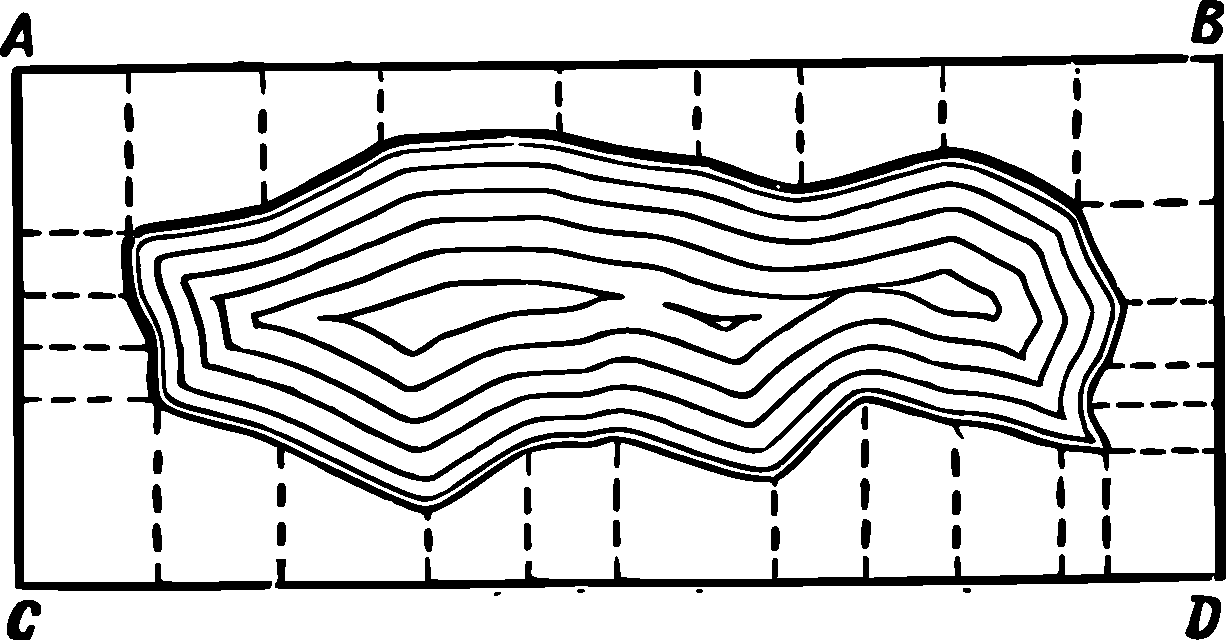
\includegraphics[width=0.8\textwidth]{figures/ch-03/fig-068.pdf}
\sidecaption{Mapping of the lake on the plan.\label{fig-068}}
\end{figure}

Additionally, using your living protractor, you can, in the absence of any tools, measure the angular height of luminaries above the horizon, the mutual separation of stars in degrees, the apparent sizes of a meteor's trail, etc. Finally, knowing how to make right angles on the ground without instruments, you can draw up a plan of a small area using the method whose essence is clear from the illustration, for example, when surveying a lake (\figr{fig-068}), measure rectangle $ABCD$, as well as the lengths of the perpendiculars dropped from prominent points on the shore, and the distances from their bases to the vertices of rectangle $ABCD$. In short, being in Robinson Crusoe's situation, knowing how to use your own hands to measure angles (and your feet to measure distances) could be useful for a variety of needs.

\section{Jacob's Staff}
\label{sec-3.8}

If you wish to have more accurate angle measures than the simple ``living protractor'' described earlier, you can make yourself a simple and convenient device that was once used by our ancestors. This is called ``Jacob's staff'' after its inventor -- a device that was widely used by sailors until the 18th century (\figr{fig-069}), before it was gradually replaced by even more convenient and precise instruments (sextants).

\begin{figure}[h!]
\centering
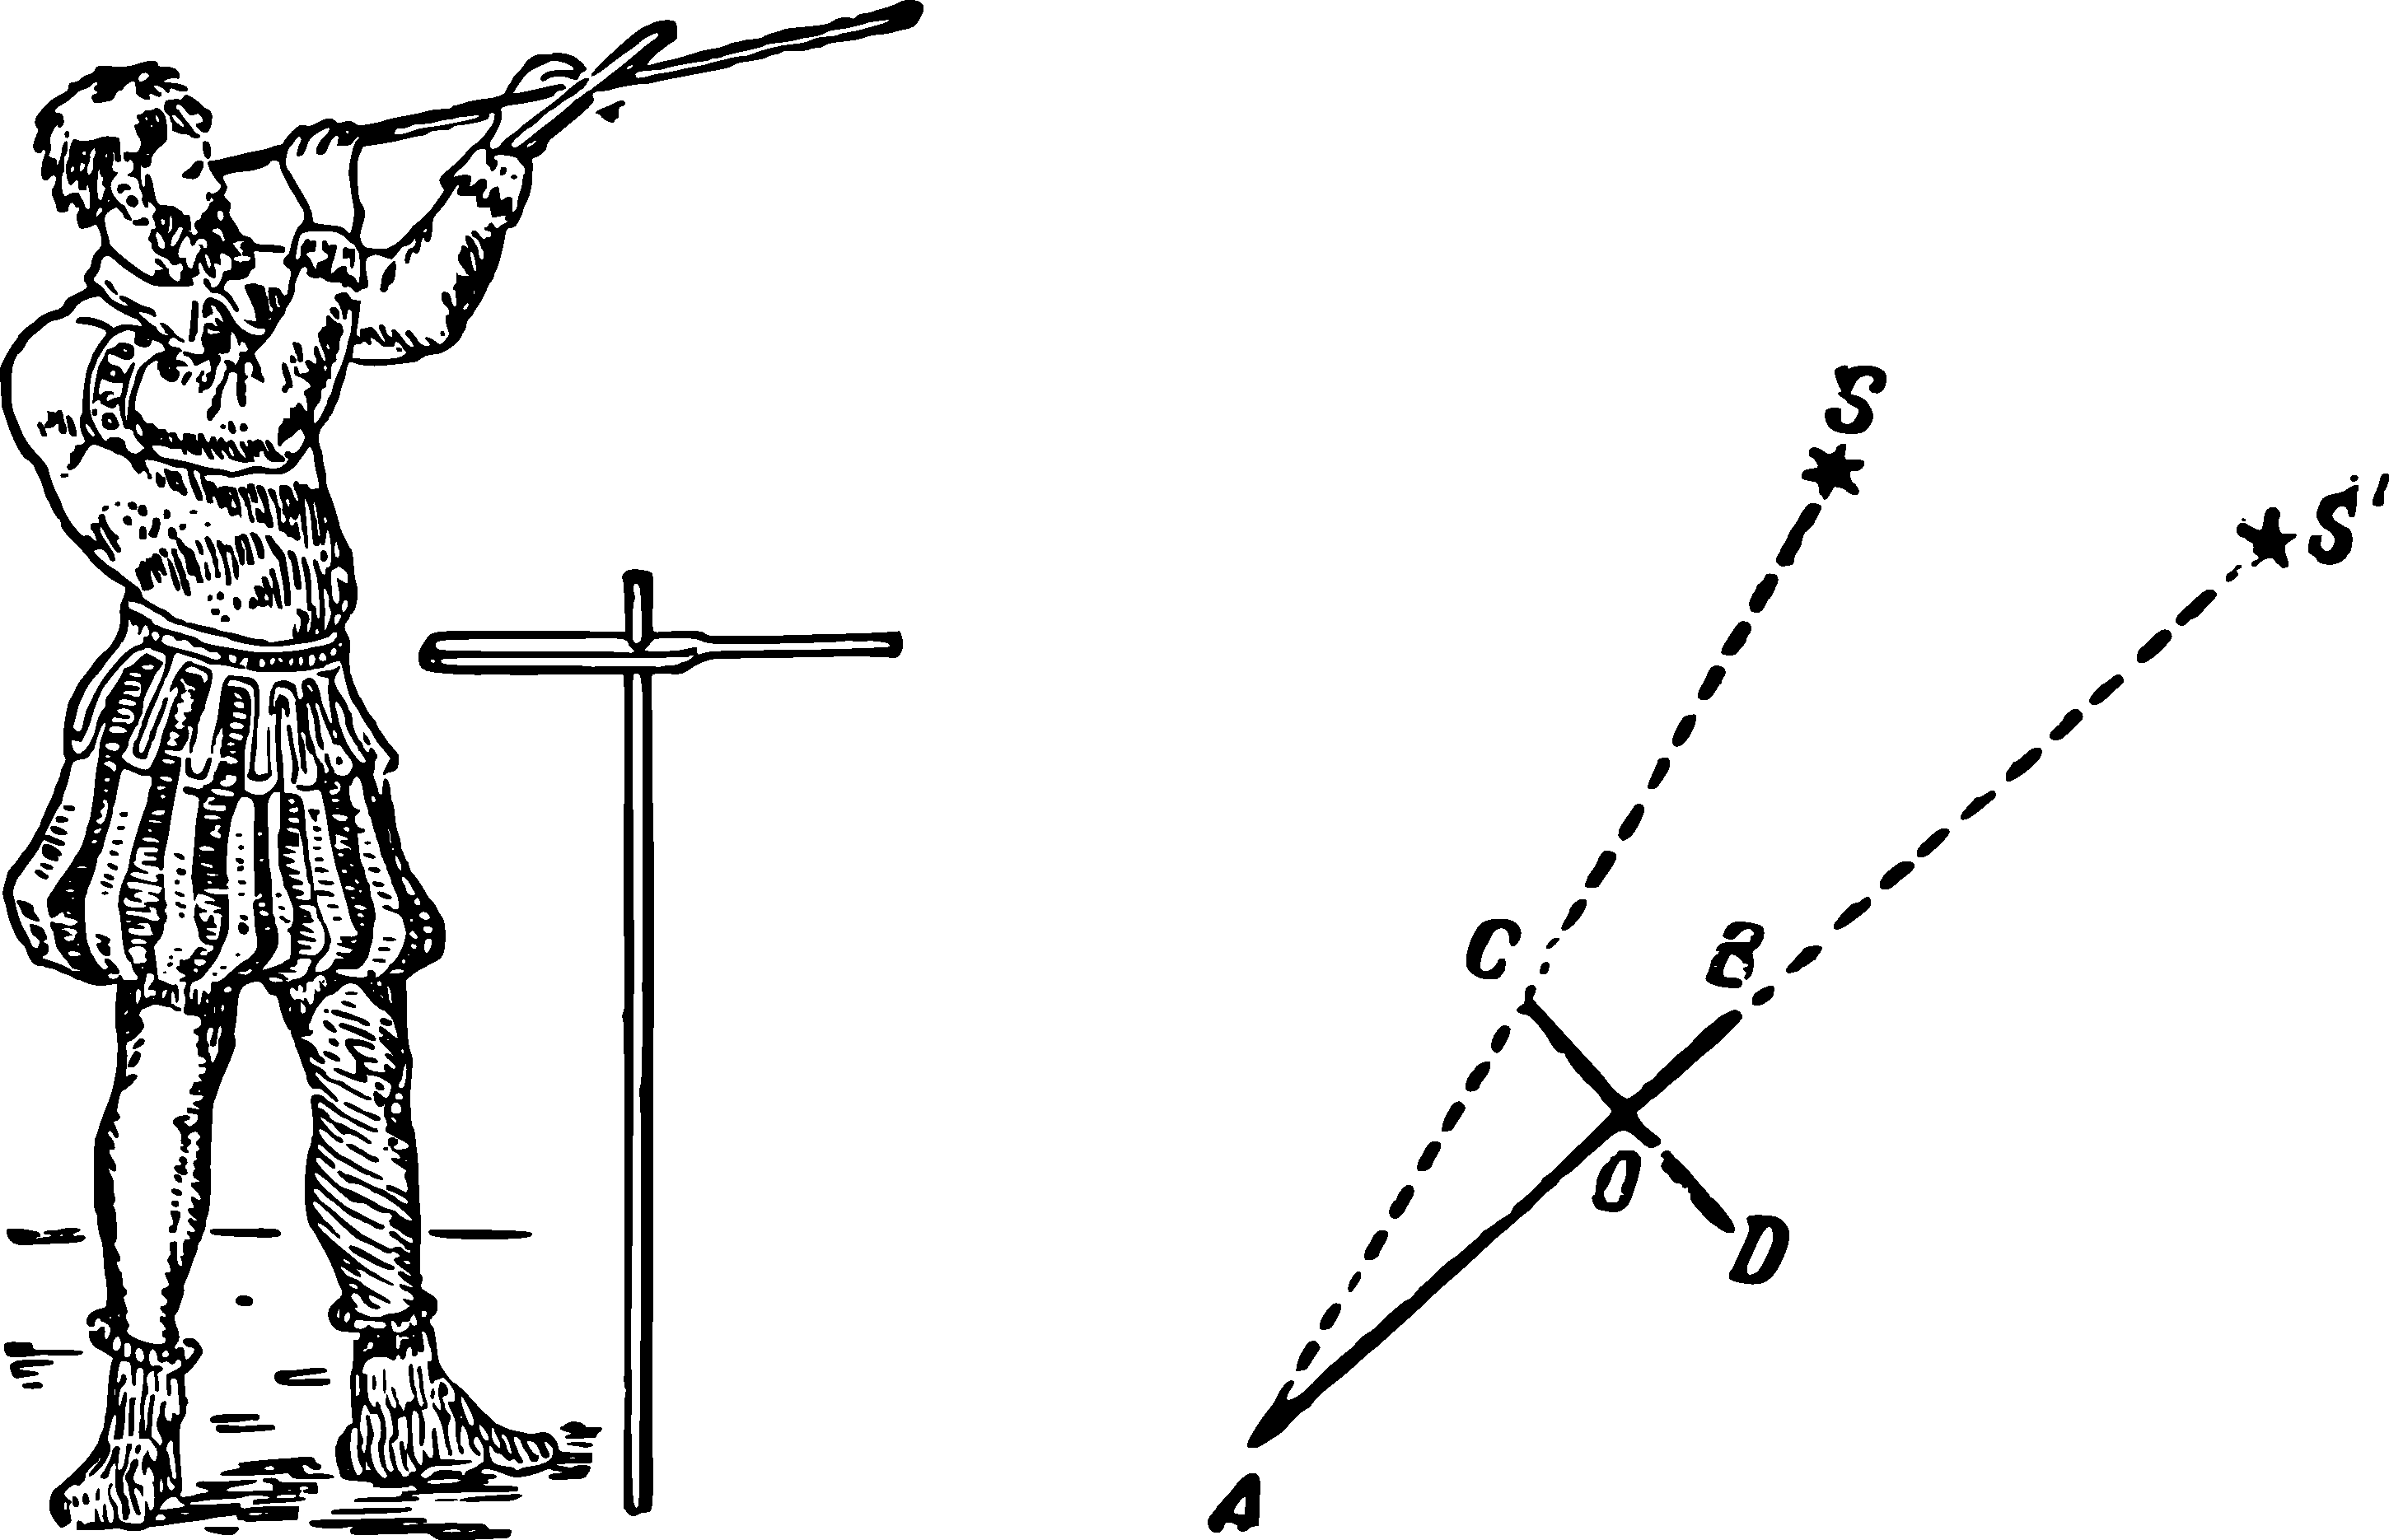
\includegraphics[width=\textwidth]{figures/ch-03/fig-069.pdf}
\sidecaption{Jacob's staff and a diagram of its use.\label{fig-069}}
\end{figure}

It consists of a long ruler $AB$, about 170–100 cm, along which a perpendicular block $CD$ can slide; both parts $CO$ and $OD$ of the sliding block are equal to each other. If you want to determine the angular distance between the stars $S$ and $S'$ using this block (\figr{fig-069}), you attach the end $A$ of the ruler to your eye (where a perforated plate is attached for convenience of observation) and direct the ruler so that the star $S'$ is visible at the end $B$ of the ruler; then you move the crosspiece $CO$ along the ruler until the star $S$ is just visible at the end $C$ (\figr{fig-069}). Now all that remains is to measure the distance $AO$ in order to calculate the value of the angle $SAS'$ using the length of the $CO$. Those familiar with trigonometry will understand that the tangent of the desired angle is equal to the ratio of $CO/AO$. Our ``field trigonometry'', presented in the fifth chapter, is also sufficient for performing this calculation: you calculate the length $AC$ using the Pythagorean theorem, then find angle $C$, whose sine is equal to $CO/AC$.

Finally, you can find the desired angle graphically; by drawing triangle $ACO$ on paper to scale, you measure angle $A$ with a protractor, or if you don't have one, by the method described in our ``field trigonometry'' (see Chapter~\ref{ch-05}).

\begin{figure}[h!]
\centering
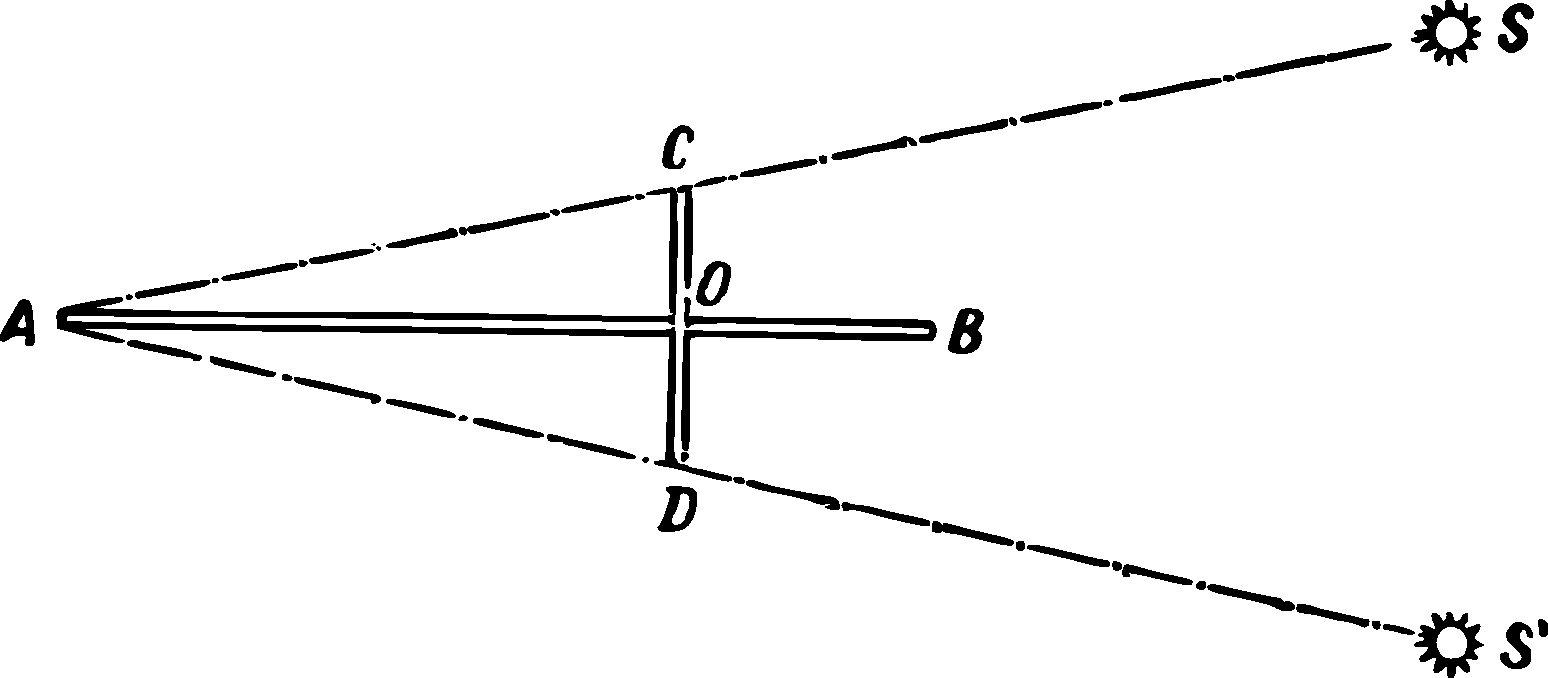
\includegraphics[width=0.9\textwidth]{figures/ch-03/fig-070.pdf}
\sidecaption{Determination of the angular distance between stars using Jacob's staff.\label{fig-070}}
\end{figure}

What is the other half of the crosspiece for? In case the angle to be measured is too large to be measured by the method described above. In that case, instead of directing the ruler $AB$ toward the star $S'$, you aim segment $AD$ toward the point $S'$, moving the crosspiece so that its end $C$ coincides with the star $S$ at the same time (\figr{fig-070}). Finding the angle $SAS'$ by calculation or construction is, of course, not difficult.

To avoid having to make calculations or constructions each time you measure, you can perform them in advance, even when making the device, and mark the results on the ruler $AB$; then, when aiming the device at the stars, you only need to read the reading recorded at point $O$ — this is the value of the measured angle.


\begin{center}
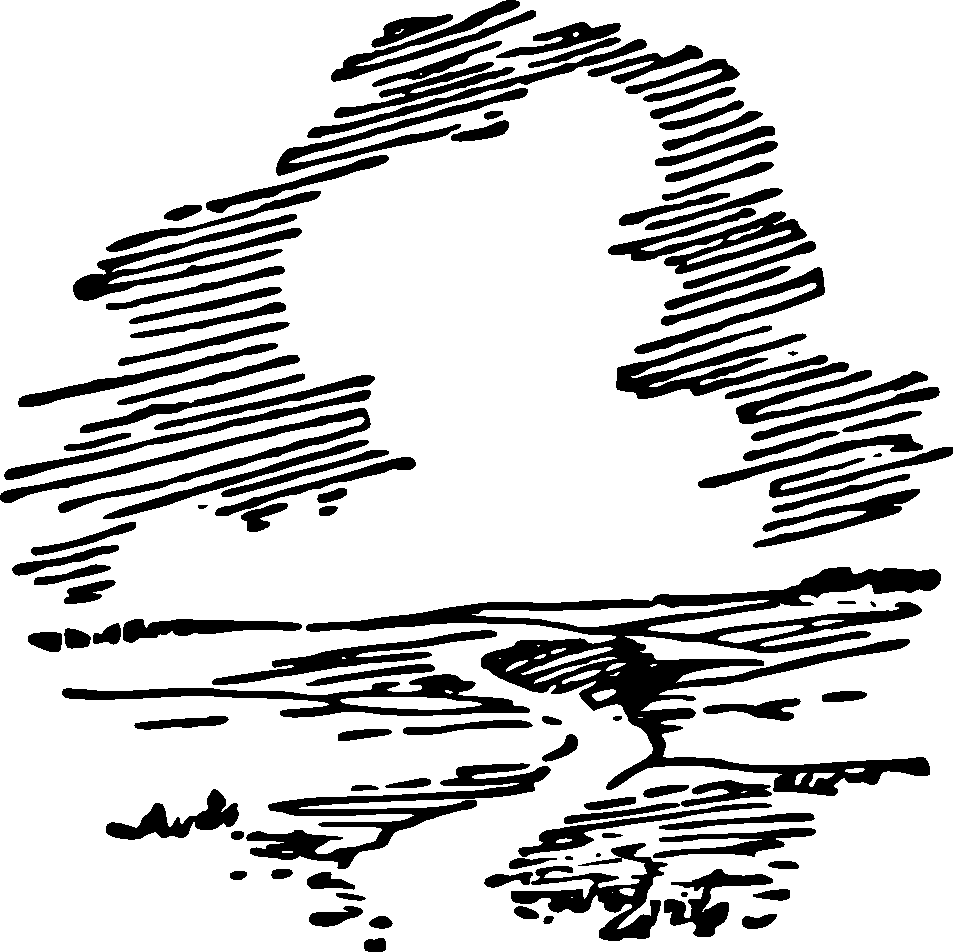
\includegraphics[width=0.3\textwidth]{figures/ch-03/fig-ch-03-tail.pdf}
\end{center}


















